% ============================================================
%  SENTINEL-GNSS — General Team Report
%  Beihang University H3I  ·  Team Pilot Project  ·  2025
%
%  Compile with: pdflatex → bibtex → pdflatex → pdflatex
%  All figures referenced relative to this file's location.
% ============================================================
\documentclass[12pt,a4paper]{article}

% -------- Encoding & fonts --------
\usepackage[T1]{fontenc}
\usepackage[utf8]{inputenc}
\usepackage{lmodern}
\usepackage{microtype}

% -------- Page layout --------
\usepackage[top=2.5cm,bottom=2.5cm,left=2.8cm,right=2.8cm]{geometry}
\usepackage{fancyhdr}
\usepackage{setspace}
\onehalfspacing

% -------- Maths --------
\usepackage{amsmath,amssymb,amsfonts}

% -------- Graphics & tables --------
\usepackage{graphicx}
\usepackage{booktabs}
\usepackage{array}
\usepackage{multirow}
\usepackage{tabularx}
\usepackage{longtable}
\usepackage{float}
\usepackage{caption}
\usepackage{subcaption}

% -------- Colours --------
\usepackage[dvipsnames]{xcolor}
\definecolor{buaaBlue}{RGB}{0,91,172}
\definecolor{buaaNavy}{RGB}{0,51,102}
\definecolor{buaaSky}{RGB}{0,160,233}
\definecolor{cleanGreen}{RGB}{76,175,80}
\definecolor{warnOrange}{RGB}{255,152,0}
\definecolor{degradRed}{RGB}{244,67,54}

% -------- Hyperlinks --------
\usepackage[colorlinks=true,linkcolor=buaaBlue,citecolor=buaaNavy,urlcolor=buaaSky]{hyperref}

% -------- References --------
\usepackage[numbers,sort&compress]{natbib}

% -------- Section heading style --------
\usepackage{titlesec}
\titleformat{\section}{\large\bfseries\color{buaaNavy}}{{\thesection}}{0.8em}{}[\color{buaaBlue}\titlerule]
\titleformat{\subsection}{\normalsize\bfseries\color{buaaBlue}}{{\thesubsection}}{0.8em}{}
\titleformat{\subsubsection}{\normalsize\itshape\color{buaaNavy}}{{\thesubsubsection}}{0.8em}{}

% -------- Page style: page number only, no running header --------
\pagestyle{plain}

% -------- Utility macros --------
\newcommand{\clean}[1]{\textcolor{cleanGreen}{\textbf{#1}}}
\newcommand{\warn}[1]{\textcolor{warnOrange}{\textbf{#1}}}
\newcommand{\degrad}[1]{\textcolor{degradRed}{\textbf{#1}}}
\newcommand{\buaa}[1]{\textcolor{buaaBlue}{\textbf{#1}}}
\newcommand{\code}[1]{\texttt{#1}}

% ============================================================
\begin{document}

% -------- Title page --------
\begin{titlepage}
  \centering
  \vspace*{1cm}
  {\color{buaaNavy}\rule{\linewidth}{2pt}}\\[0.5cm]
  {\normalsize\color{buaaBlue} SENTINEL-GNSS}\\[0.25cm]
  {\LARGE\bfseries\color{buaaNavy} AI-Based Proactive Prediction of GNSS\\[0.2cm]
   Signal Degradation for Autonomous\\[0.4cm]
   Vehicle Navigation}\\[0.45cm]
  {\large\color{buaaBlue} Group Report}\\[0.5cm]
  {\color{buaaNavy}\rule{\linewidth}{2pt}}\\[1.5cm]

  {\large\bfseries Team Pilot Project}\\[0.5cm]

  \begin{tabular}{ll}
    \toprule
    \textbf{Member} & \textbf{Student ID} \\
    \midrule
    Ojerinde Joel          & LS2525253 \\
    Ogunlade Joshua        & LS2525237 \\
    Mustapha Ibrahim       & LS2525238 \\
    Ingeriyinkindi Claudine & LS2525236 \\
    Rashid Md Harun Or     & LS2525219 \\
    \bottomrule
  \end{tabular}\\[1.5cm]

  {\large Hangzhou International Institute of Innovation (H3I), Beihang University}\\[0.3cm]
  {\large Regional Centre for Space Science and Technology Education}\\[0.15cm]
  {\large in Asia and the Pacific (RCSSTEAP)}\\[0.3cm]
  {\large Hangzhou, China · 2026}\\[2cm]

  \begin{minipage}{0.85\textwidth}
    \centering
    \itshape
    Submitted in partial fulfilment of the requirements for the \\
    Pilot Project module, Hangzhou International Institute of Innovation (H3I),
    Beihang University.
  \end{minipage}
\end{titlepage}

% -------- Abstract --------
\begin{abstract}
Reliable absolute positioning is a safety-critical requirement for autonomous vehicles.
Global Navigation Satellite System (GNSS) receivers provide this positioning but are
vulnerable to silent degradation in urban environments due to Non-Line-of-Sight (NLOS)
multipath and signal blockage from buildings.
Existing monitoring approaches, including RTKLIB quality codes, RAIM, and recent
machine-learning classifiers, are \emph{reactive}: they report degradation only after it
has affected positioning performance, giving the vehicle zero preparation time.

This report describes \buaa{SENTINEL-GNSS}, a Transformer-LSTM neural network that
\emph{predicts} GNSS signal degradation 5, 15, and 30 seconds before it occurs.
The model processes a 30-second sliding window of 37 receiver-derived features and
outputs a three-class forecast (\clean{CLEAN} / \warn{WARNING} / \degrad{DEGRADED})
for each prediction horizon in a single forward pass.

Trained on 149,662 labelled epochs from Beihang University field collections and the
UrbanNav Hong Kong dataset, the model achieves a Macro-F1 of \textbf{0.821} at the
+5\,s horizon with a DEGRADED-class recall of \textbf{0.847}.
Critically, when evaluated on the fully held-out city of Tokyo, SENTINEL retains a
DEGRADED-class F1 of \textbf{0.75} where the strongest classical baseline
(RandomForest) collapses to \textbf{0.15}, demonstrating transferable urban degradation
representations.

The prediction is integrated into a 9-state Extended Kalman Filter (EKF) via adaptive
measurement noise covariance, producing a 48.8\,\% reduction in positioning RMSE during
degraded epochs on the Trimble Shinjuku dataset.
The learned prediction, after an unsupervised receiver-domain calibration, reaches
38.7\,\%, and an online estimator of the degraded noise scale raises this to 43.2\,\%
without manual tuning.
A Huber-robust EKF and a Bootstrap Particle Filter with Student-\emph{t} GPS likelihood
are also evaluated, with the Particle Filter achieving a 40.1\,\% degraded-segment gain
on the Odaiba open-harbour scenario.
A live, multilingual dashboard visualises all fusion tracks in real time.
\end{abstract}

\newpage
\tableofcontents


\newpage
\listoffigures

\newpage
\listoftables
\newpage

% ============================================================
\section{Introduction}
\label{sec:intro}
% ============================================================

Autonomous vehicles (AVs) depend on accurate, continuous positioning to execute safety-critical
decisions at road speed.
A vehicle travelling at 60\,km/h covers 17 metres per second; a positioning gap of even
5 seconds can place a vehicle in the wrong lane, miss a junction, or trigger emergency braking
at the wrong location.
Among the positioning sensors available to AVs—cameras, LiDAR, radar, and Inertial Measurement
Units (IMU)—GNSS remains the sole source of drift-free absolute position \cite{groves2013gnss}.

The fundamental problem is that GNSS \emph{fails silently} in dense urban environments.
NLOS multipath caused by building reflections introduces position errors of 10--200\,m into
the receiver solution, yet the receiver continues to report a ``valid'' fix with no indication
of the error magnitude \cite{zhu2018gnss}.
Existing quality monitors—RTKLIB solution quality codes, Receiver Autonomous Integrity
Monitoring (RAIM) \cite{brown1997raim}, and recent supervised classifiers \cite{liu2023gnss,hsu2018nlos}—are
reactive: they identify degradation at the moment it begins.
At 60\,km/h this gives the vehicle controller zero preparation time.

\subsection{Contributions of This Work}

This paper makes the following contributions:

\begin{enumerate}
  \item \textbf{Problem reformulation.} We reframe GNSS quality monitoring as a
    \emph{predictive} rather than reactive problem, and demonstrate that 5--30\,s lead
    times are achievable with a learned sequence model.

  \item \textbf{SENTINEL-GNSS architecture.} A unified Transformer--LSTM network with
    three output heads ($+5$\,s, $+15$\,s, $+30$\,s) achieves Macro-F1\,=\,0.821 at the
    +5\,s horizon using 1.46\,M parameters and runs at 0.0449\,ms per sample.

  \item \textbf{Cross-city generalisation.} Training on Beihang + Hong Kong and evaluating
    on fully held-out Tokyo, the network maintains DEGRADED-class F1\,=\,0.753 while the
    strongest classical baseline (RandomForest) drops to 0.148.

  \item \textbf{Prediction-informed sensor fusion.} Integration of SENTINEL predictions
    into an adaptive EKF yields a 48.8\,\% degraded-RMSE improvement on a clean dual-frequency
    receiver (Trimble Shinjuku), 25.2\,\% on a single-frequency u-blox receiver (Huber EKF),
    and 40.1\,\% on an open-harbour scenario (Student-\emph{t} PF).

  \item \textbf{Open benchmark.} A multi-city, multi-receiver labelled dataset of 149,662
    epochs across 4 cities and 9+ receiver types is released with the paper.
\end{enumerate}

Figure~\ref{fig:problem} contrasts the reactive and the proactive approach, and
Figure~\ref{fig:pipeline} shows the full system that delivers the proactive behaviour.

\begin{figure}[H]
  \centering
  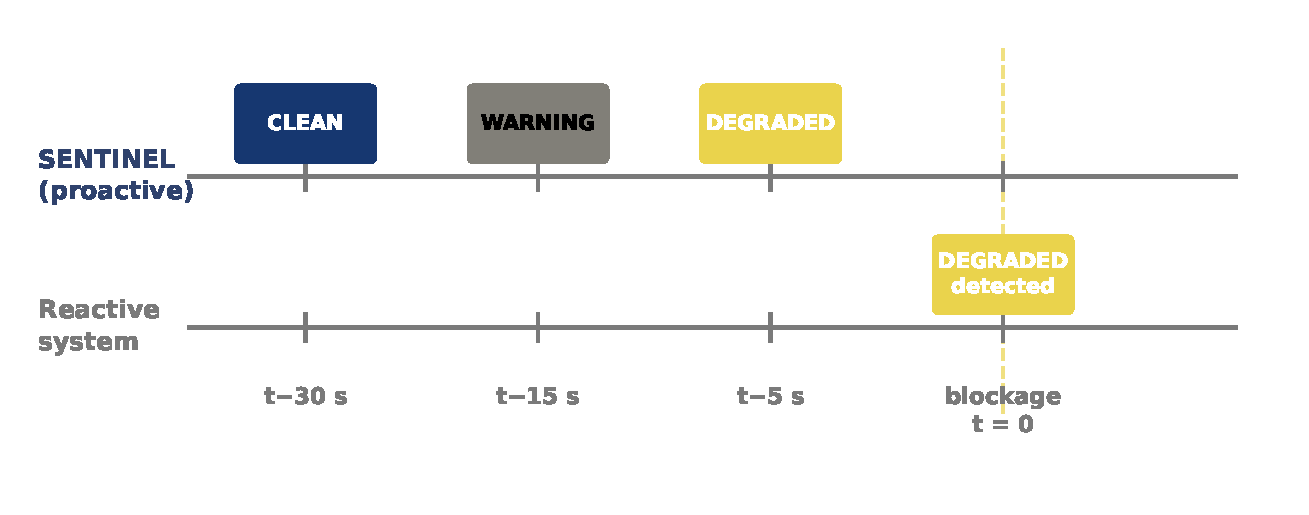
\includegraphics[width=0.92\textwidth]{../../results/paper_figures/fig13_reactive_vs_proactive.pdf}
  \caption{Reactive monitoring against the proactive SENTINEL-GNSS approach. A reactive
           system detects the failure only after it occurs, with no warning window. The
           proactive system gives a 30 second early warning, pre-activates dead reckoning,
           and maintains navigation through the outage.}
  \label{fig:problem}
\end{figure}

\begin{figure}[H]
  \centering
  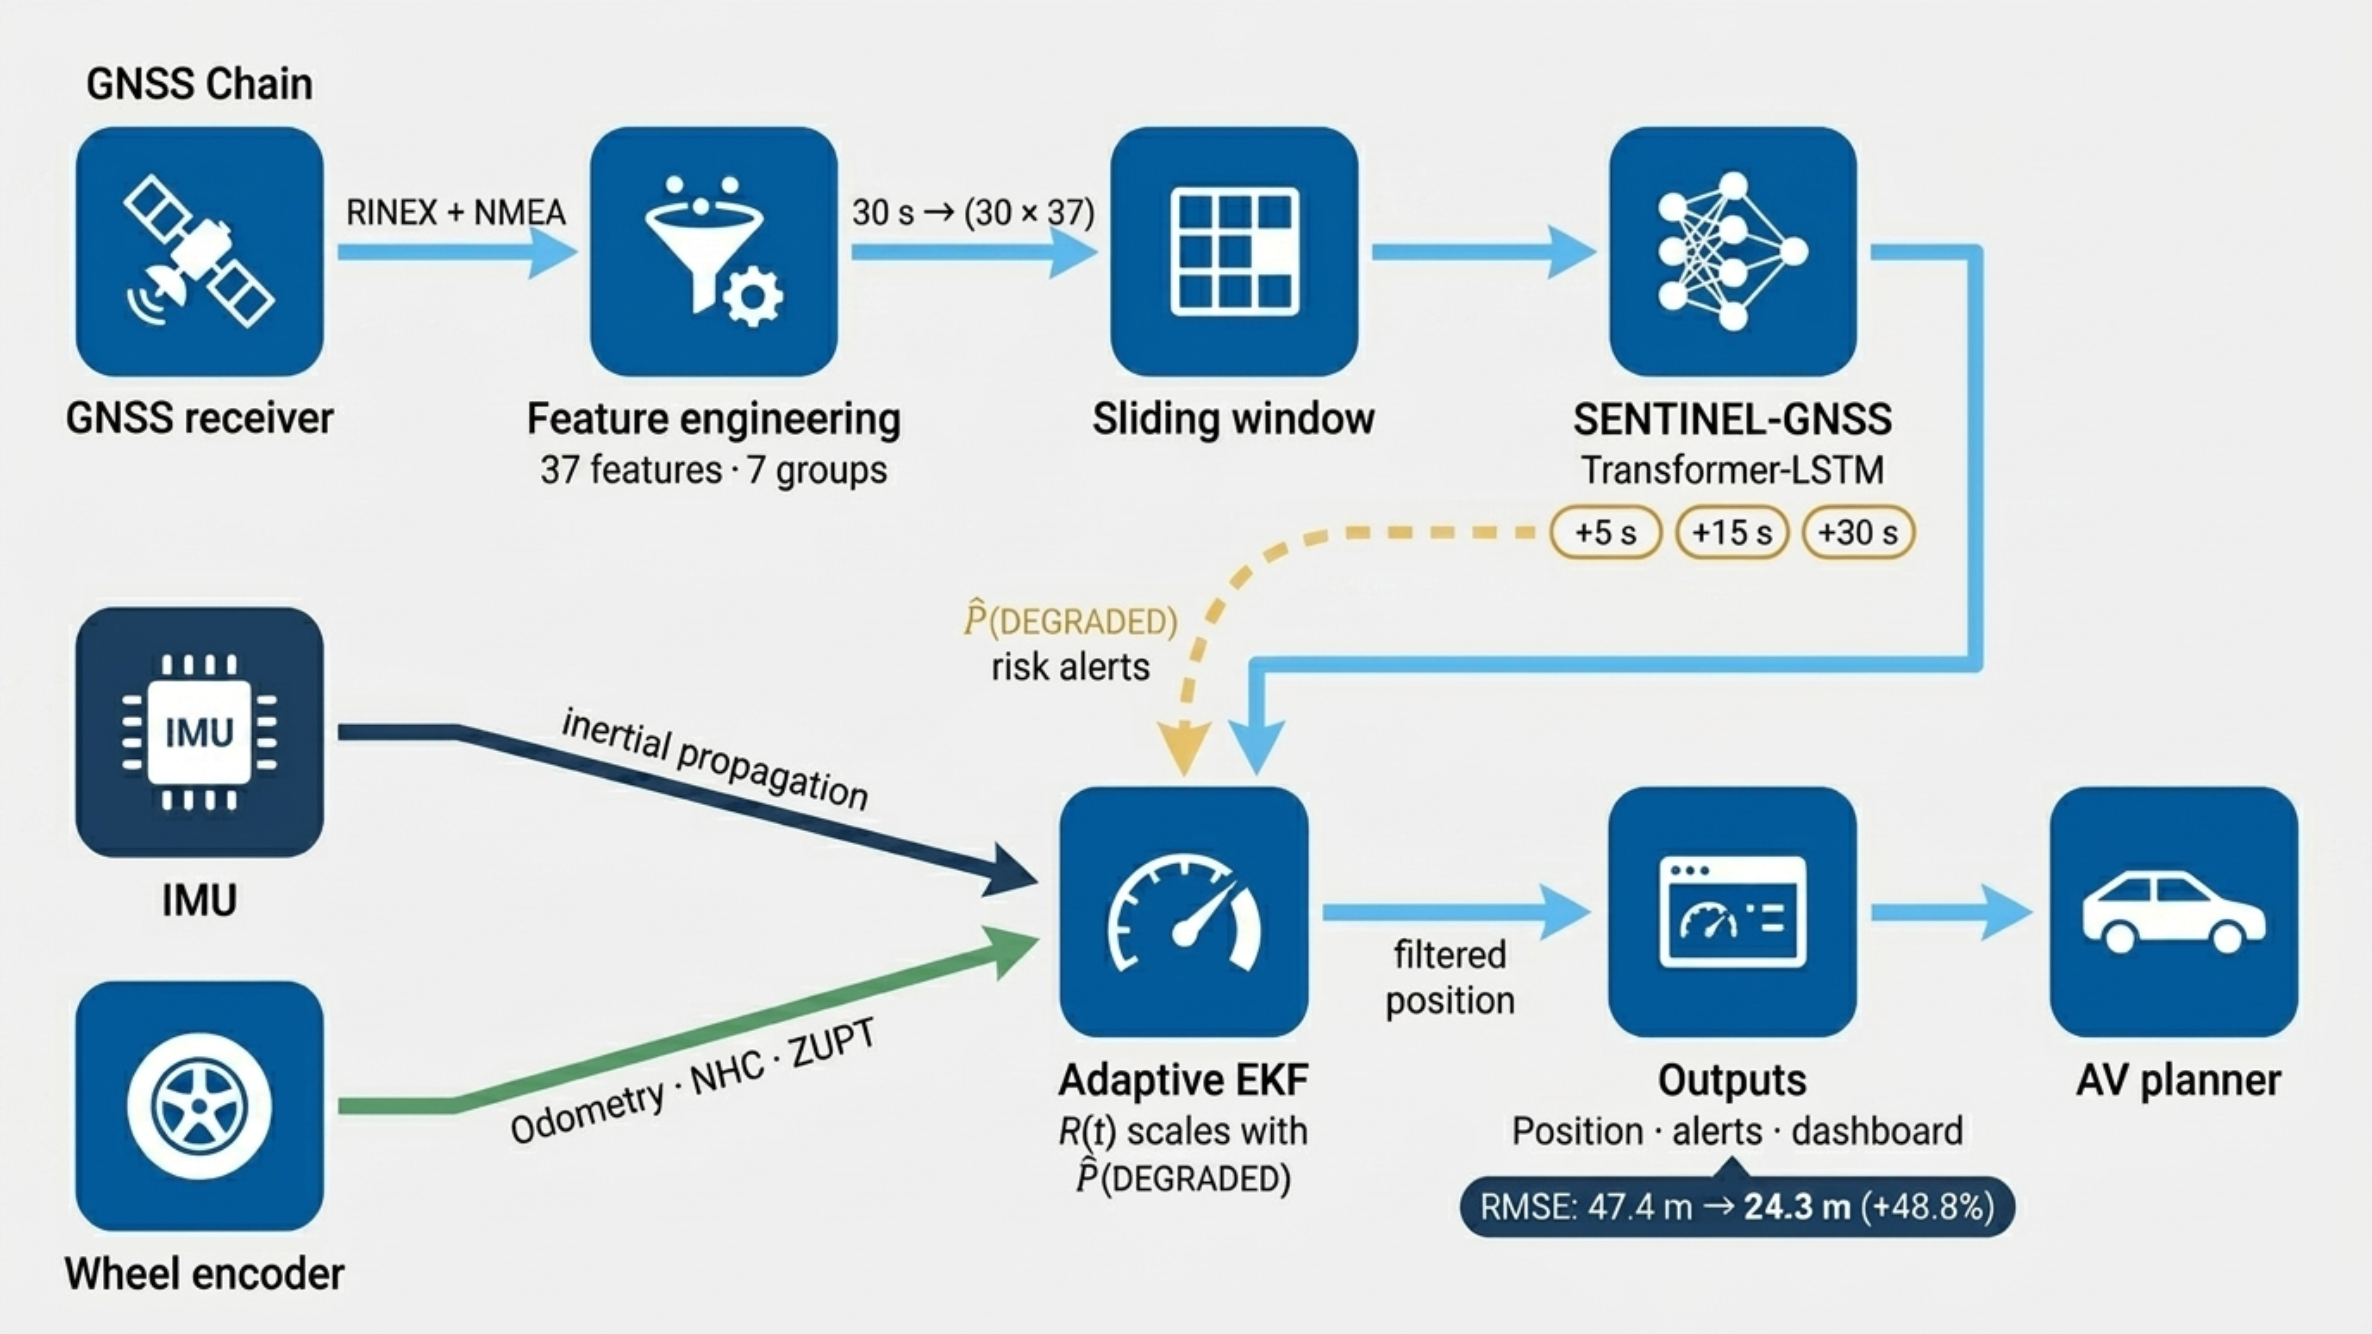
\includegraphics[width=0.97\textwidth]{../system_pipeline.png}
  \caption{End to end SENTINEL-GNSS system. Sensors feed feature engineering, the model
           forecasts the degradation probability at three horizons, the Extended Kalman
           Filter scales its measurement noise with that probability, and the output layer
           produces position, alerts, and the dashboard view.}
  \label{fig:pipeline}
\end{figure}

\newpage
% ============================================================
\section{Related Work}
\label{sec:related}
% ============================================================

\subsection{GNSS Quality Monitoring}

Traditional GNSS integrity monitoring is based on RAIM \cite{brown1997raim}, which uses
pseudorange consistency checks to detect and isolate faulty satellites.
RAIM is well-understood and widely deployed but operates purely on the current epoch;
it provides no forward-looking indication of approaching degradation.
RTKLIB \cite{rtklib} assigns solution quality codes (Q=1 fix, Q=5 float) which are
commonly used as degradation indicators in research, but these again reflect current
rather than future quality.

\subsection{Machine Learning for GNSS}

Chen \emph{et al.}~\cite{chen2019gps} demonstrated that recurrent networks could classify
GNSS signal quality using C/N$_0$ time series, achieving accuracy above 90\,\% on
simulated data.
Liu \emph{et al.}~\cite{liu2023gnss} applied gradient-boosted trees to multi-feature
GNSS classification in Hong Kong urban environments, reporting strong in-domain results.
These works are \emph{contemporaneous classifiers}: they label the current epoch as
clean or degraded.
SENTINEL differs in that it predicts the class of a \emph{future} epoch, turning
quality monitoring into a forecasting problem.

\subsection{Adaptive Kalman Filtering}

The Mehra (1970) innovation-based adaptive R estimator \cite{mehra1970} is a classical
approach to unknown measurement noise covariance.
However, in urban NLOS environments it fails catastrophically: GPS and the filter
co-drift, producing artificially small innovations that cause R to shrink, increasing
Kalman gain and accelerating drift (we measured RMSE $>238{,}000$\,m in testing).
Prediction-based R inflation, as proposed here, sidesteps this identification problem
by conditioning R adaptation on a learned classifier output rather than the innovation
sequence.

% ============================================================
\section{Dataset and Feature Engineering}
\label{sec:data}
% ============================================================

\subsection{Data Sources}

The training dataset comprises three sources:

\begin{enumerate}
  \item \textbf{Beihang field collections.} Five controlled scenarios (A--E) collected
    on campus using a Septentrio Mosaic-X5C receiver:
    (A) instantaneous signal blockage, (B) urban canyon traverse,
    (C) partial tree canopy obstruction, (D) open-sky baseline,
    (E) gradual building approach.

  \item \textbf{UrbanNav Hong Kong.} Public dataset from Hong Kong Polytechnic University
    \cite{hsu2021urbannav} covering Medium, Deep, Harsh, and Tunnel urban environments
    with 9+ receiver types and RTK ground truth at centimetre accuracy.

  \item \textbf{UrbanNav Tokyo (held-out).} Shinjuku (Trimble RTKLIB SPP + u-blox F9P)
    and Odaiba (u-blox F9P) drives, excluded from all training and validation.
    Used exclusively for cross-city evaluation and EKF experiments.
\end{enumerate}

The combined labelled dataset contains \textbf{149,662 epochs} across 4 cities and 9+
receiver types.
The three-class label schema (CLEAN / WARNING / DEGRADED) was applied uniformly:
CLEAN when positioning error $<2$\,m and mean C/N$_0 > 35$\,dB-Hz;
DEGRADED when error $> 5$\,m, C/N$_0 < 30$\,dB-Hz, or satellite count $< 4$;
WARNING otherwise.

\begin{figure}[H]
  \centering
  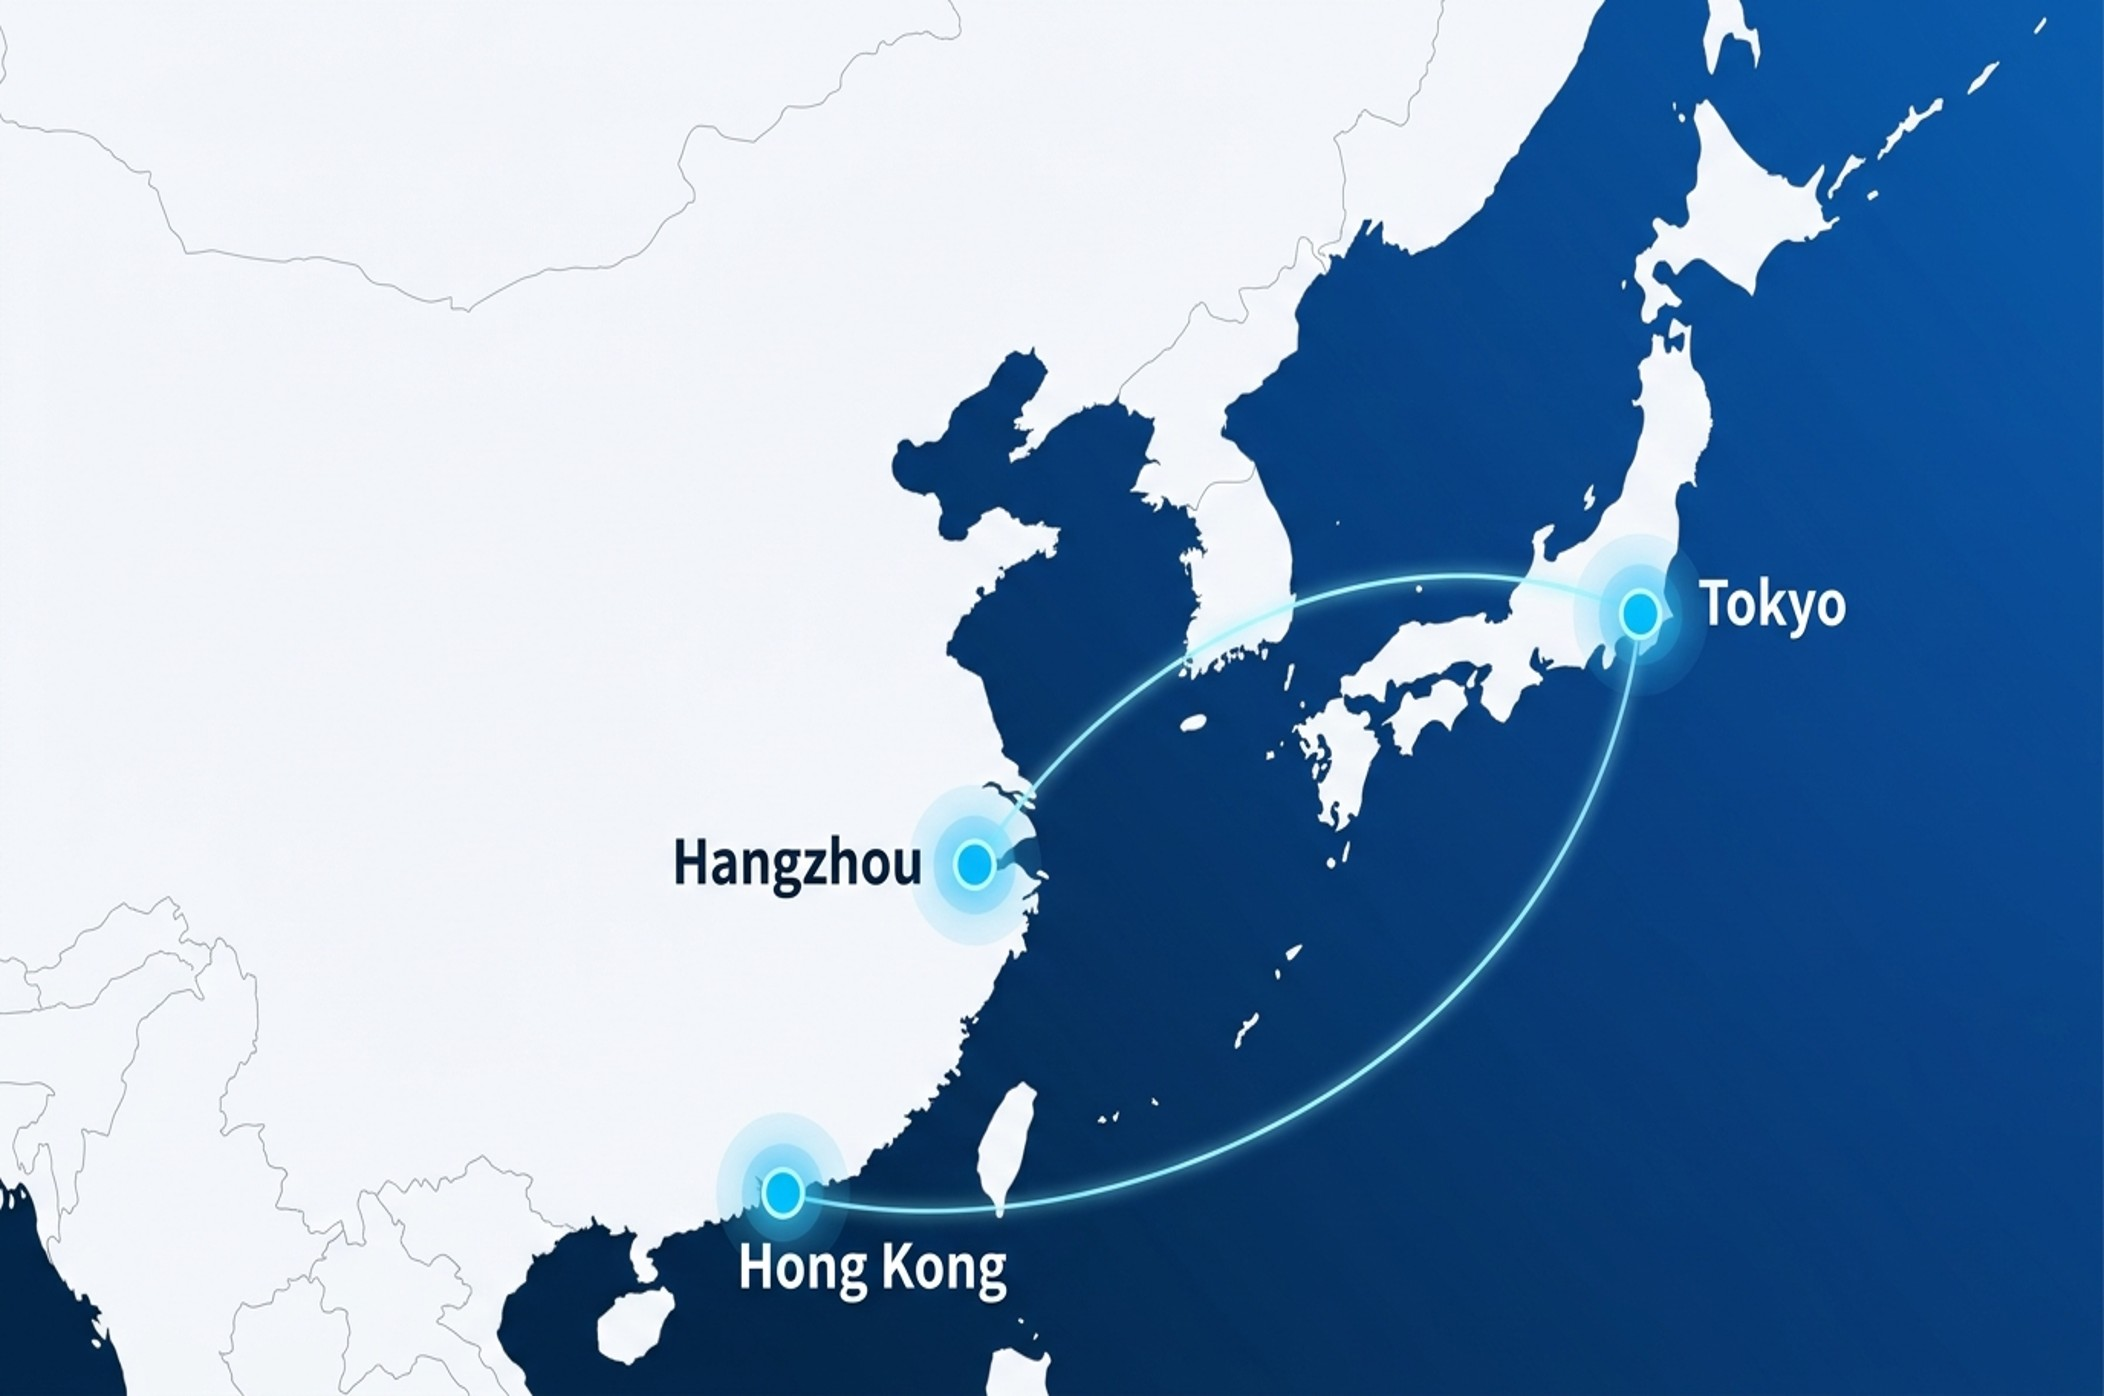
\includegraphics[width=0.74\textwidth]{../data_3_sources.jpg}
  \caption{The three evaluation cities. Hangzhou and Hong Kong are used for training and
           in-domain testing. Tokyo is held out for the cross-city test and the EKF
           experiments.}
  \label{fig:cities}
\end{figure}

\subsection{Feature Engineering}

Raw RINEX and NMEA observables are processed through RTKLIB \cite{rtklib} to produce
\textbf{37 features} per epoch in seven groups (33 signal features plus four derived
inputs: \texttt{cnr\_available}, \texttt{pdop\_delta}, \texttt{hdop\_delta},
\texttt{receiver\_tier}). Geographic coordinates are excluded from model inputs to
prevent route-specific overfitting.

\begin{description}
  \item[Position quality (3)] Altitude (\texttt{alt}) and horizontal position standard deviations (\texttt{lat\_std}, \texttt{lon\_std}) from RTKLIB north/east error estimates.
  \item[Signal strength / C/N$_0$ (6)] Mean, minimum, maximum, standard deviation, and linear trend of C/N$_0$ across tracked satellites, plus a binary availability flag (\texttt{cnr\_available}).
  \item[Satellite count (5)] Number of satellites used in the SPP solution, mean and minimum count over the window, visibility ratio, and satellite drop rate.
  \item[DOP geometry (7)] PDOP, HDOP, VDOP, GDOP, and horizontal-to-vertical DOP ratio (\texttt{dop\_ratio}), plus first-order differences $\Delta$PDOP and $\Delta$HDOP to capture the rate of geometry change.
  \item[Receiver status (6)] Normalised solution quality, baseline satellite count, solution age, fix continuity fraction, fix transition count, and hardware quality tier (\texttt{receiver\_tier}).
  \item[Temporal patterns (5)] Position variance, C/N$_0$ variance, elevation violations, multipath proxy, and clock bias over the 30-s window.
  \item[Atmospheric effects (5)] Ionospheric delay, tropospheric delay, cycle slip count, and pseudorange residual mean and standard deviation.
\end{description}

Features are $z$-score normalised using training-set statistics only.

\subsection{Sliding Window Construction}

A causal sliding window of $W = 30$ epochs (30\,s at 1\,Hz) produces input tensors
of shape $(30 \times 37)$.
Labels are assigned at horizons $h \in \{5, 15, 30\}$\,s after the last observed epoch,
giving three binary-per-class prediction targets per window.
The train/validation/test split follows session boundaries (70/15/15) to prevent
temporal leakage.

\begin{figure}[H]
  \centering
  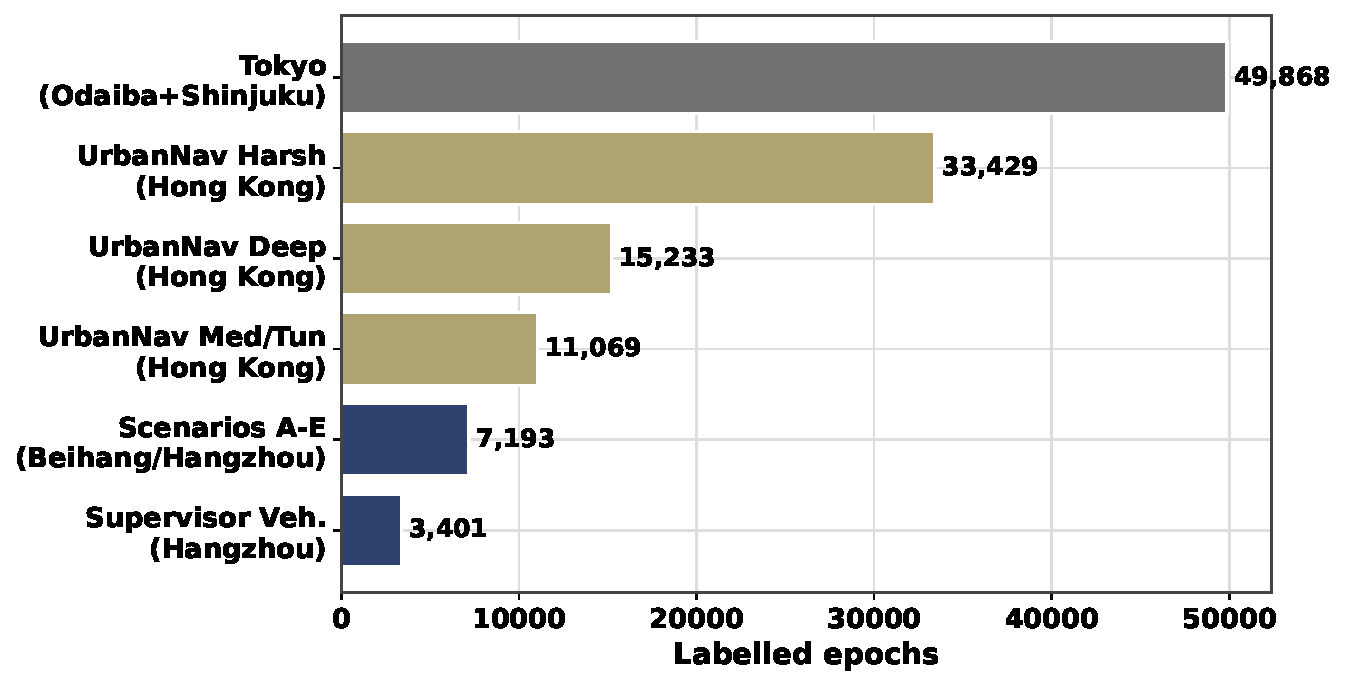
\includegraphics[width=0.70\textwidth]{../../results/paper_figures/fig10_dataset_composition.pdf}
  \caption{Dataset composition across sources, cities, and receiver types.
           The Tokyo split is strictly held-out for cross-city evaluation.}
  \label{fig:dataset}
\end{figure}

\begin{figure}[H]
  \centering
  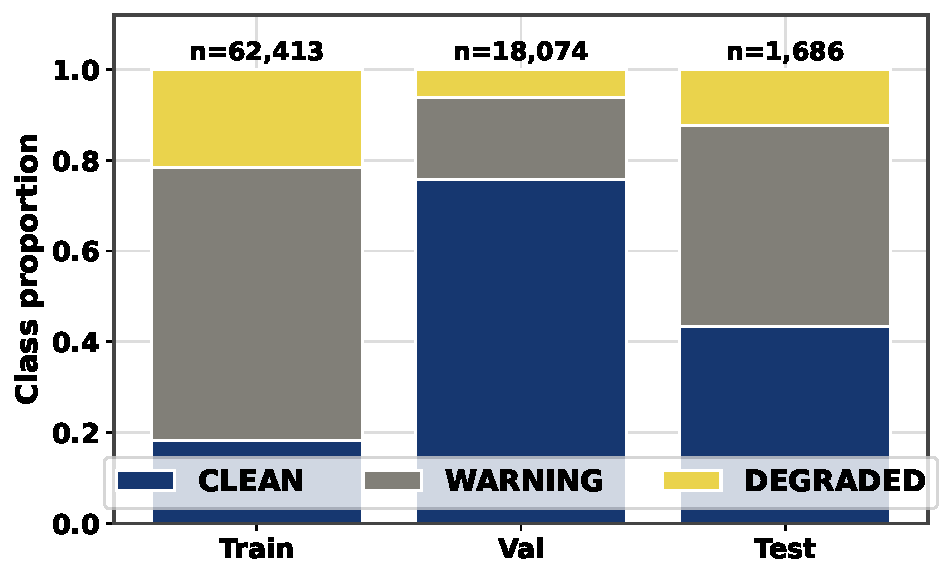
\includegraphics[width=0.70\textwidth]{../../results/paper_figures/fig11_class_distribution.pdf}
  \caption{Class distribution per data split. DEGRADED is the minority class
           (7.8\,\% of training windows), handled by focal loss and class weighting.}
  \label{fig:class_dist}
\end{figure}

% ============================================================
\section{SENTINEL-GNSS Architecture}
\label{sec:method}
% ============================================================

\subsection{Model Architecture}

SENTINEL-GNSS is a hybrid Transformer--LSTM network designed to exploit two
complementary temporal scales:

\begin{itemize}
  \item \textbf{Global dependencies (Transformer).} Satellite rising/setting events and
    PDOP trends that recur across a 30-second window are captured by multi-head self-attention
    \cite{vaswani2017attention}, which can directly relate distant timesteps without
    gradient decay.

  \item \textbf{Sequential dynamics (LSTM).} The directional approach to a degradation
    event (C/N$_0$ gradually declining, pseudorange residuals growing) is captured by a
    stacked two-layer LSTM \cite{hochreiter1997lstm} which maintains a hidden state summarising
    the trajectory within the window.
\end{itemize}

The architecture (1.46\,M parameters) is:

\begin{equation}
  \mathbf{x}_{1:T} \xrightarrow{\text{Linear + PE}}
  \mathbf{h}^\mathrm{T}_{1:T} \xrightarrow{\text{TransEnc}}
  \mathbf{h}^\mathrm{T}_{T} \xrightarrow{\text{LSTM}}
  \mathbf{h}^\mathrm{L}_T \xrightarrow{\text{FC}_h}
  \hat{y}^{(h)},\quad h \in \{5,15,30\}
\end{equation}

where the Transformer encoder has $d_\mathrm{model}=128$, 8 heads, 2 layers,
feedforward dimension $d_\mathrm{ff}=512$, dropout 0.3;
and the LSTM has hidden dimension 256, 2 stacked layers.
A shared auxiliary head over the LSTM output regularises against dataset shift.

\subsection{Training Protocol}

\begin{itemize}
  \item \textbf{Loss.} Focal loss \cite{lin2017focal} with $\gamma=1.0$ and class weights
    $[1, 2, 5]$ for \{CLEAN, WARNING, DEGRADED\}.
    No SMOTE applied to the network (imbalance handled at the loss level; SMOTE applied
    only for tree baselines).
  \item \textbf{Optimiser.} AdamW \cite{kingma2014adam}, $\text{lr}=10^{-3}$,
    weight decay $10^{-4}$, cosine annealing \cite{loshchilov2017cosine}.
  \item \textbf{Early stopping.} Patience 20 epochs on validation Macro-F1.
  \item \textbf{Framework.} PyTorch \cite{paszke2019pytorch}.
    Best checkpoint: epoch 10, Val-F1\,=\,0.861.
    Training converged in 65 epochs.
\end{itemize}

\begin{figure}[H]
  \centering
  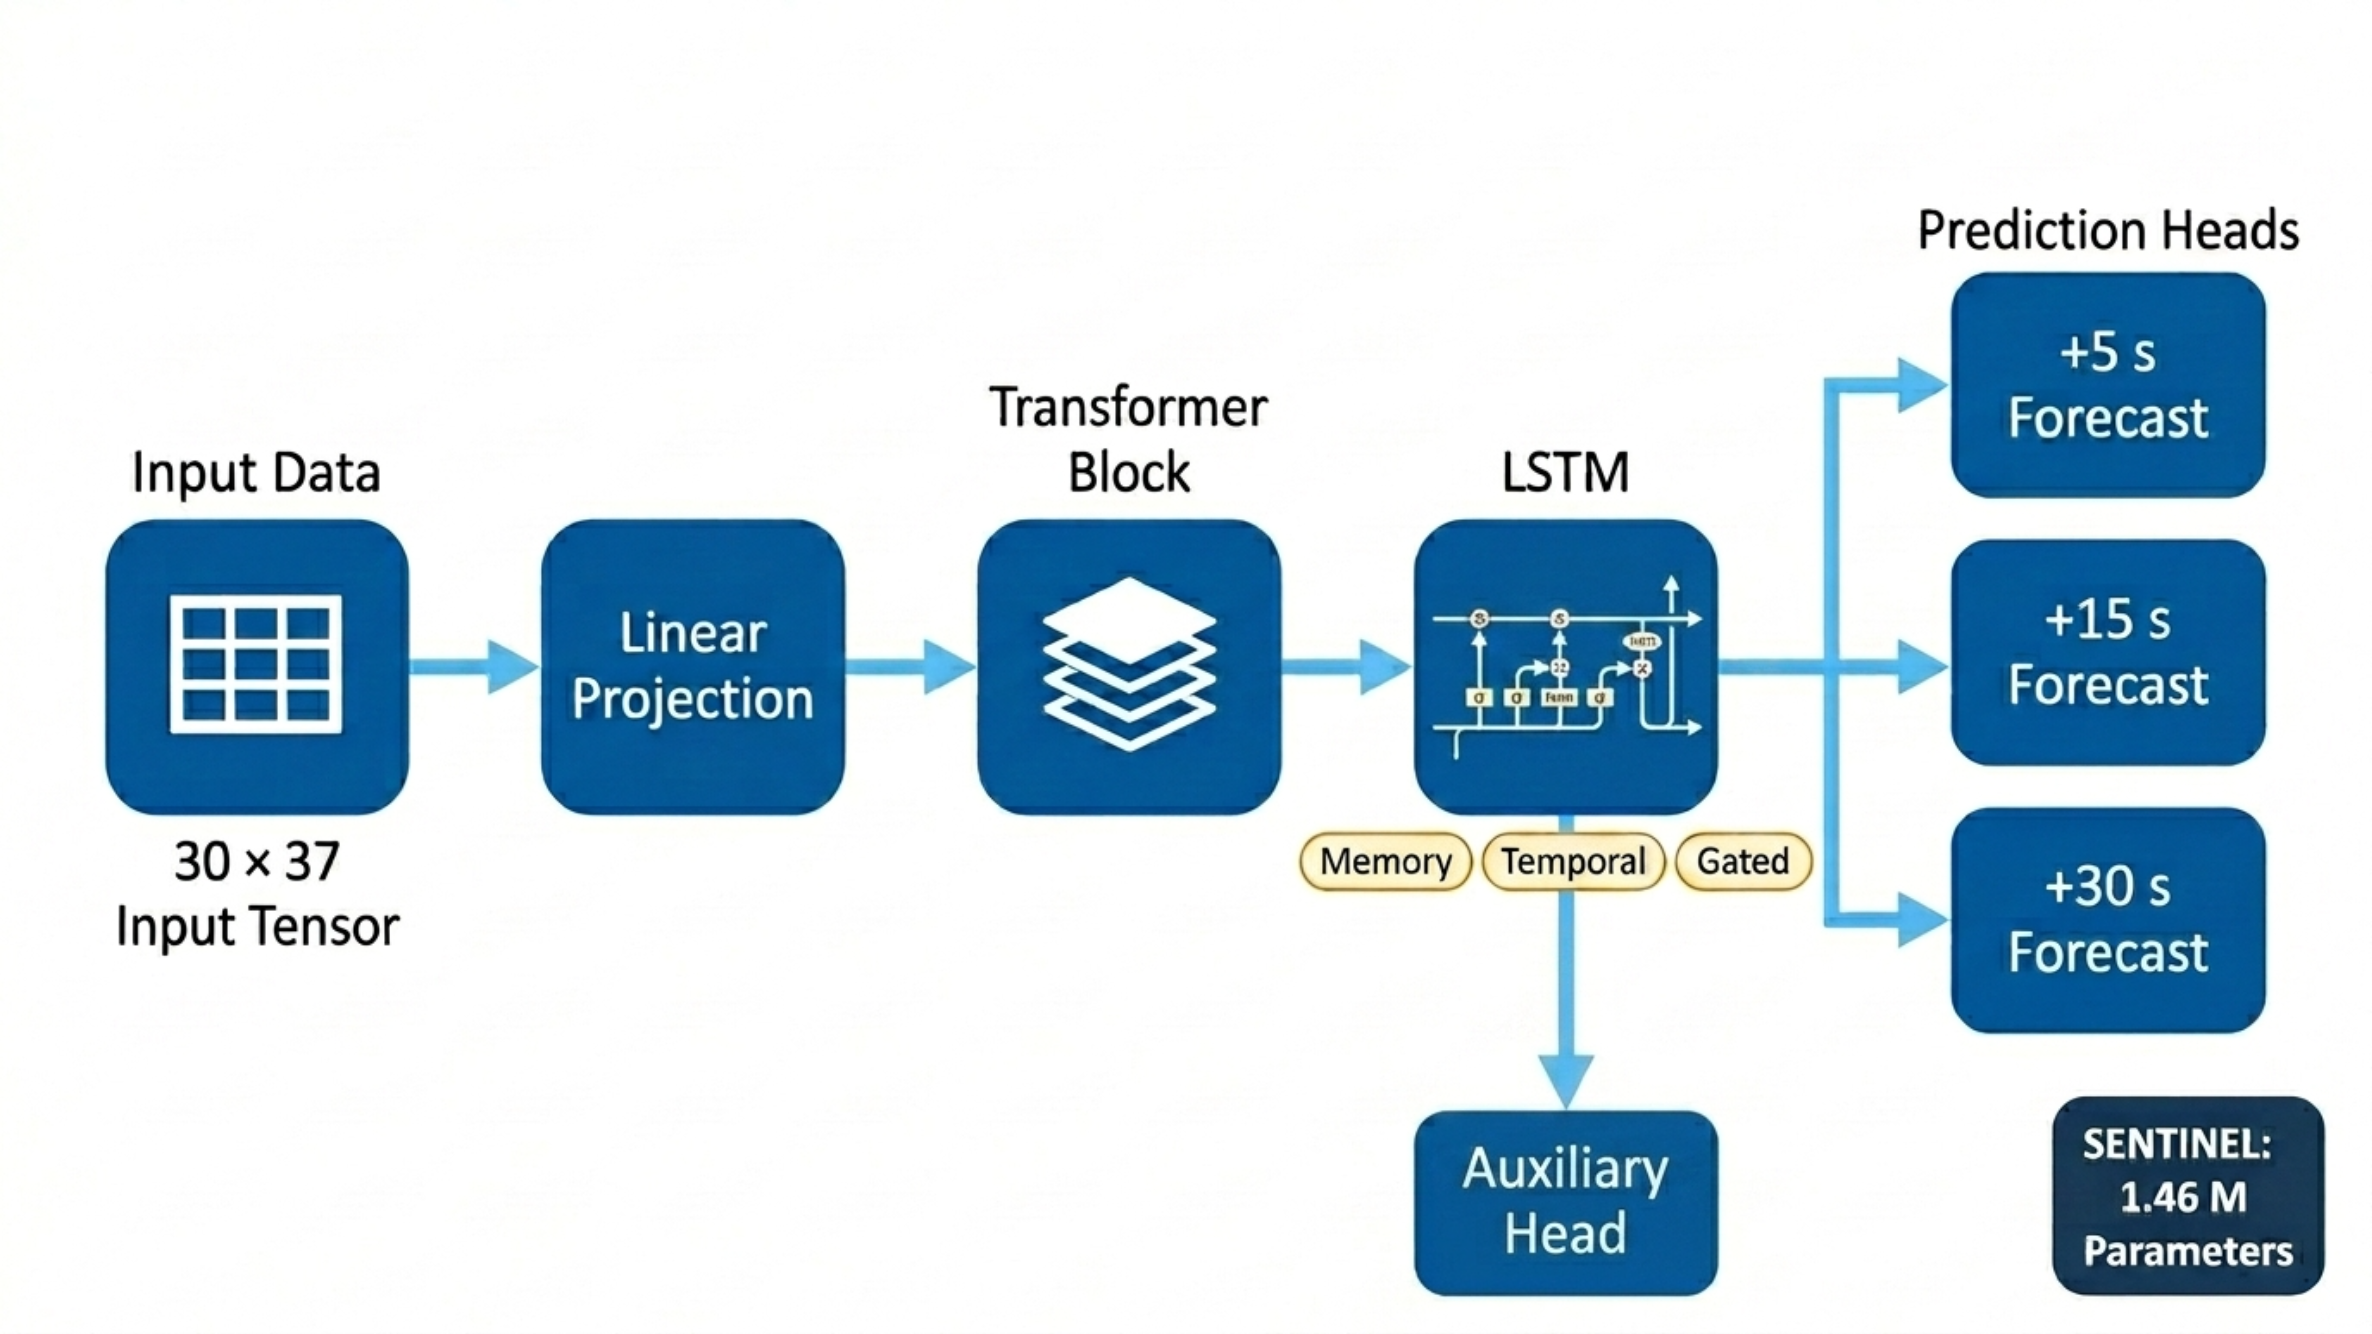
\includegraphics[width=0.98\textwidth]{../inside_gnss.png}
  \caption{SENTINEL-GNSS architecture. A linear projection and positional encoding map the
           30 by 37 input window to dimension 128. A two-layer Transformer encoder reads the
           window, a two-layer recurrent encoder with 256 hidden units summarises the
           sequence, and three heads output the class probabilities at the 5, 15, and 30
           second horizons. The model has 1.46 million parameters.}
  \label{fig:arch}
\end{figure}



% ============================================================
\section{Results}
\label{sec:results}
% ============================================================

\subsection{Multi-Horizon Classification Performance}

Table~\ref{tab:multihorizon} shows the held-out test results for all three prediction
horizons.

\begin{table}[H]
  \centering
  \caption{SENTINEL-GNSS multi-horizon test performance (held-out test set,
           $n = 1{,}686$ windows). 95\,\% confidence intervals from 1,000 bootstrap
           iterations.}
  \label{tab:multihorizon}
  \begin{tabular}{lcccl}
    \toprule
    \textbf{Horizon} & \textbf{Accuracy} & \textbf{Macro-F1} & \textbf{MCC} &
    \textbf{95\,\% CI (Macro-F1)} \\
    \midrule
    $+5$\,s  & 0.853 & \textbf{0.821} & 0.773 & [0.800,\;0.843] \\
    $+15$\,s & 0.789 & 0.741 & 0.691 & [0.717,\;0.764] \\
    $+30$\,s & 0.830 & 0.783 & 0.731 & [0.758,\;0.804] \\
    \bottomrule
  \end{tabular}
\end{table}

\begin{table}[H]
  \centering
  \caption{Per-class performance at the $+5$\,s horizon.
           High DEGRADED recall (0.847) is the priority for AV safety.}
  \label{tab:perclass}
  \begin{tabular}{lcccc}
    \toprule
    \textbf{Class} & \textbf{Precision} & \textbf{Recall} & \textbf{F1} &
    \textbf{Support} \\
    \midrule
    \clean{CLEAN}   & 0.868 & 0.993 & 0.927 & 731 \\
    \warn{WARNING}  & 0.947 & 0.718 & 0.817 & 746 \\
    \degrad{DEGRADED} & 0.623 & 0.847 & \textbf{0.718} & 209 \\
    \bottomrule
  \end{tabular}
\end{table}

\begin{figure}[H]
  \centering
  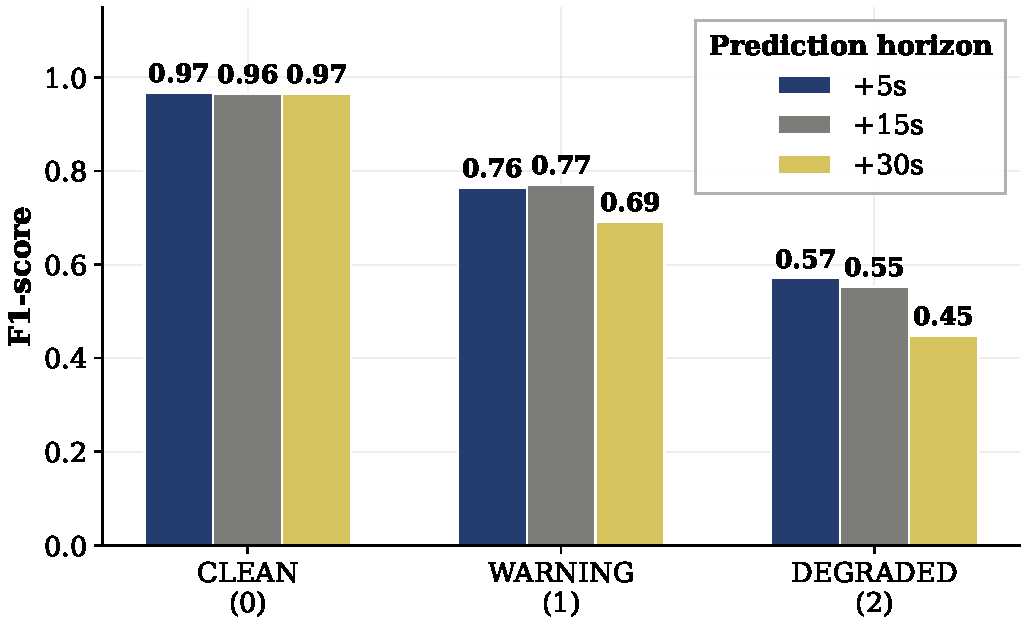
\includegraphics[width=\textwidth]{../../results/paper_figures/multi_horizon_comparison.pdf}
  \caption{Multi-horizon Macro-F1 and per-class F1 comparison across all three
           prediction horizons. The $+5$\,s horizon achieves the strongest DEGRADED-class
           F1 and is used for real-time EKF integration.}
  \label{fig:multihorizon}
\end{figure}

\begin{figure}[H]
  \centering
  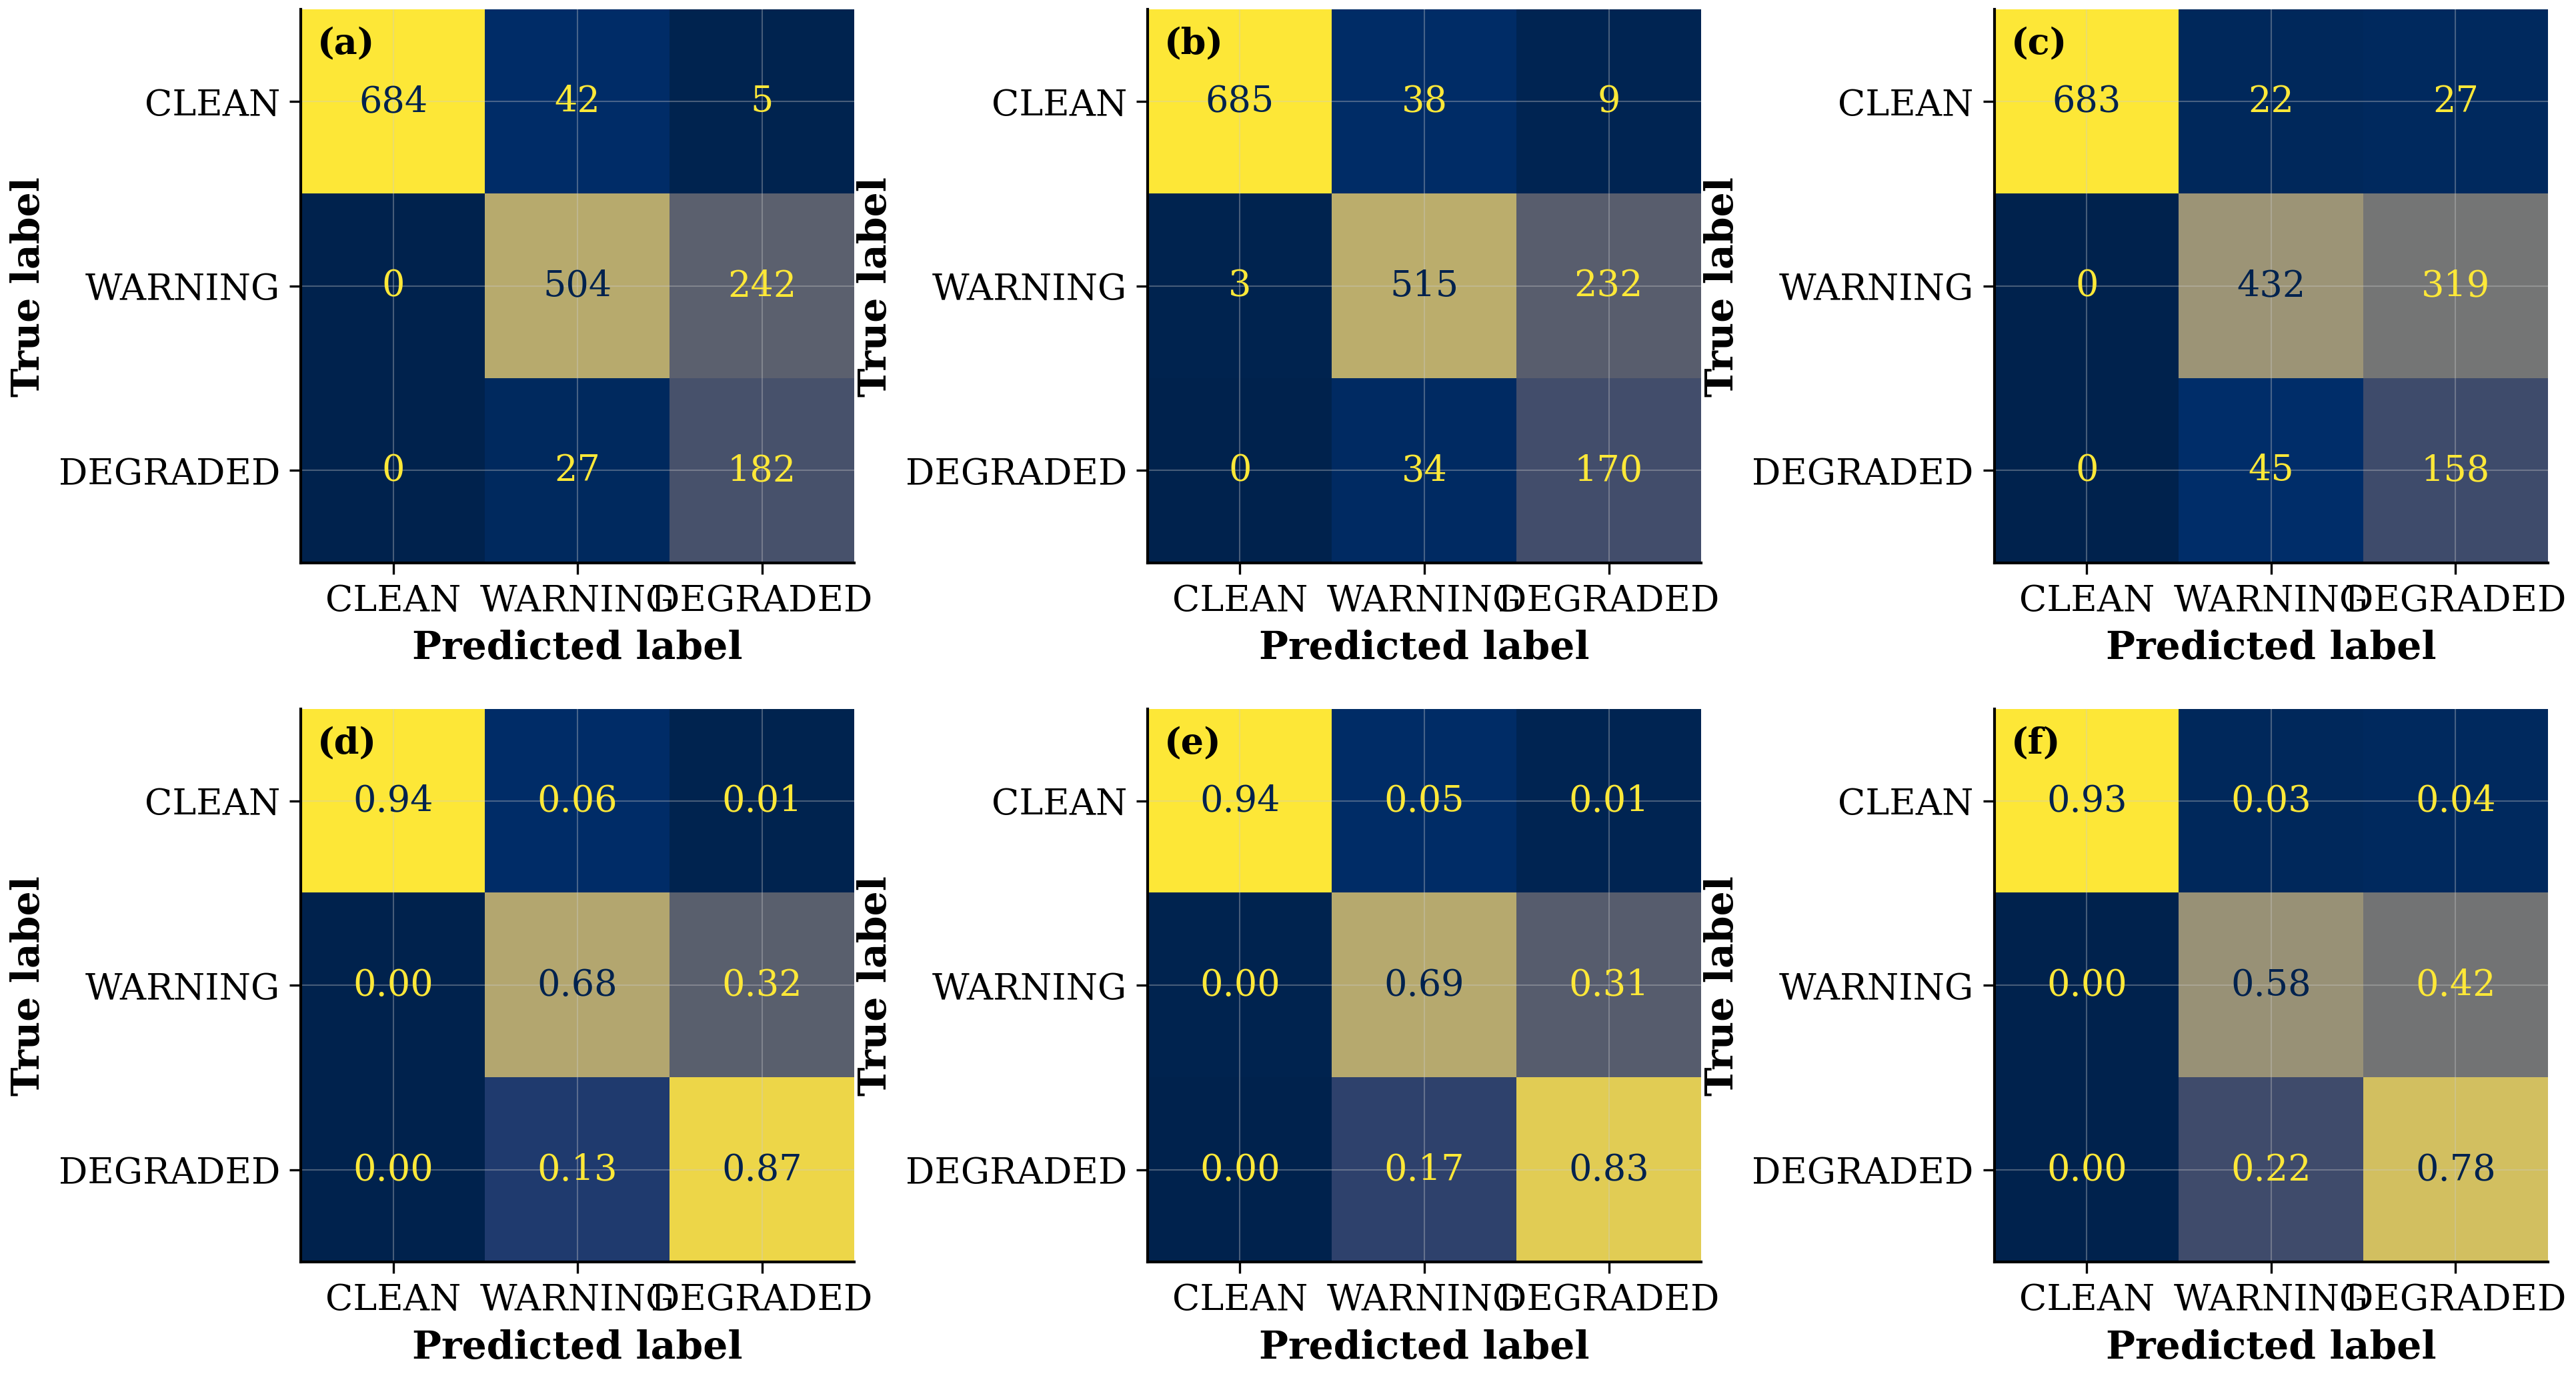
\includegraphics[width=\textwidth]{../../results/paper_figures/confusion_matrices_test.png}
  \caption{Confusion matrices for all three prediction horizons on the held-out test set.
           The $+5$\,s matrix shows strong DEGRADED recall with limited clean/warning
           confusion.}
  \label{fig:confusion}
\end{figure}

\subsection{Ablation Study}

Table~\ref{tab:ablation} confirms that both the Transformer and the LSTM contribute
to performance.

\begin{table}[H]
  \centering
  \caption{Ablation results at the $+5$\,s horizon. The full Transformer+LSTM
           model outperforms all single-component variants.}
  \label{tab:ablation}
  \begin{tabular}{lcccc}
    \toprule
    \textbf{Architecture} & \textbf{Params} & \textbf{Macro-F1} & \textbf{MCC} &
    \textbf{DEGRADED F1} \\
    \midrule
    Transformer-only & 0.43\,M & 0.767 & 0.725 & 0.571 \\
    LSTM-only      & 1.03\,M & 0.767 & 0.702 & 0.645 \\
    \textbf{Full (Trans+LSTM)} & \textbf{1.46\,M} &
      \textbf{0.821} & \textbf{0.773} & \textbf{0.718} \\
    \bottomrule
  \end{tabular}
\end{table}

The Transformer alone over-flags DEGRADED (precision 0.42); the LSTM provides
directional sequential context that suppresses false alarms.
The LSTM alone under-detects DEGRADED (recall 0.645 vs 0.847); the Transformer
captures the longer-range satellite geometry changes that precede degradation.

\begin{figure}[H]
  \centering
  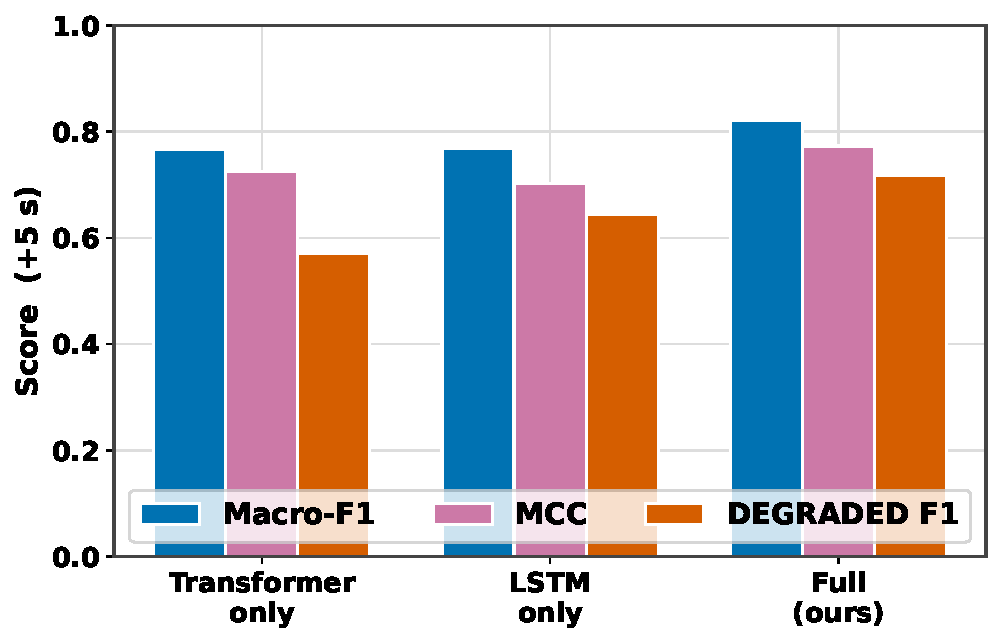
\includegraphics[width=0.75\textwidth]{../../results/paper_figures/fig04_ablation.pdf}
  \caption{Ablation study: Macro-F1, MCC, and DEGRADED-class F1 for each architecture
           variant. Each component contributes independently.}
  \label{fig:ablation}
\end{figure}

\subsection{Cross-City Generalisation}

\begin{table}[H]
  \centering
  \caption{Cross-city generalisation. Training: Beihang + Hong Kong. Test: Tokyo
           (entirely excluded from training). The DL model retains safety-critical
           DEGRADED-class F1 that the RF model cannot.}
  \label{tab:crosscity}
  \begin{tabularx}{\textwidth}{l>{\centering\arraybackslash}X>{\centering\arraybackslash}X>{\centering\arraybackslash}c>{\centering\arraybackslash}X}
    \toprule
    \textbf{Model} & \textbf{Beihang Macro-F1} & \textbf{Tokyo Macro-F1} &
    \textbf{Gap} & \textbf{Tokyo DEGRADED F1} \\
    \midrule
    \textbf{SENTINEL (DL)} & 0.822 & 0.649 & $-0.173$ &
      \textbf{\textcolor{cleanGreen}{0.75}} \\
    RandomForest           & 0.926 & 0.618 & $-0.308$ &
      \textbf{\textcolor{degradRed}{0.15}} \\
    \bottomrule
  \end{tabularx}
\end{table}

The 5$\times$ difference in Tokyo DEGRADED F1 (0.75 vs 0.15) is the central result.
RandomForest memorises city-specific C/N$_0$ thresholds and satellite count values;
SENTINEL learns a transferable sequence representation that generalises across urban
building geometries and receiver types.

\begin{figure}[H]
  \centering
  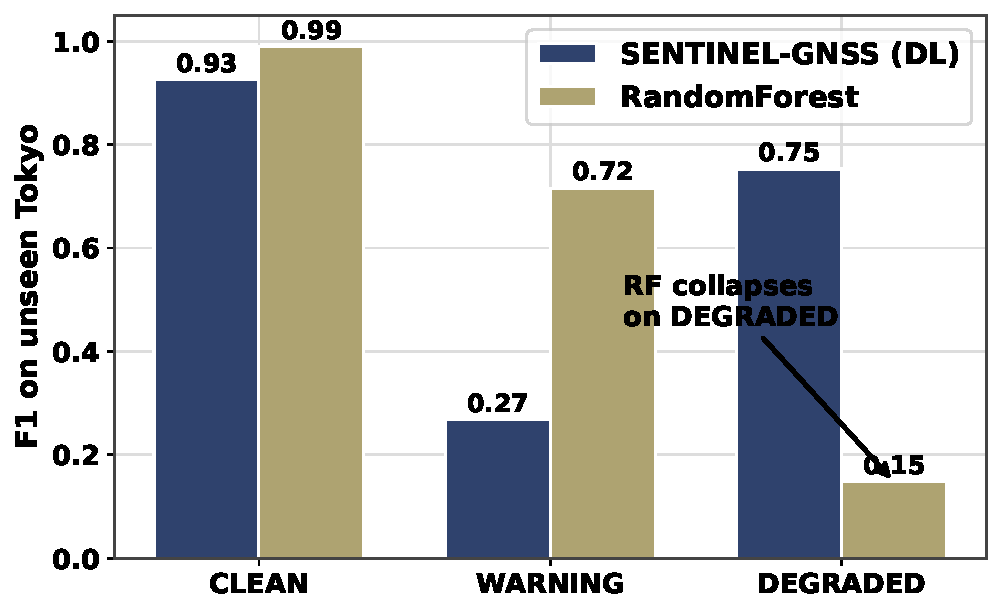
\includegraphics[width=0.72\textwidth]{../../results/paper_figures/fig05_crosscity_degraded.pdf}
  \caption{Cross-city DEGRADED-class F1 comparison. The DL model transfers to the
           unseen city; the RF baseline collapses, demonstrating the superiority of
           learned sequential representations for cross-environment generalisation.}
  \label{fig:crosscity}
\end{figure}

\subsection{Prediction-Informed EKF Fusion}

\subsubsection{System Design}

At each epoch, the SENTINEL $+5$\,s DEGRADED probability is used to select the GPS
measurement noise covariance:
\begin{equation}
  \mathbf{R} = \begin{cases}
    r_\mathrm{deg}^2 \mathbf{I}_2 & \text{if } P(\text{DEGRADED}) > 0.45 \\
    r_\mathrm{base}^2 \mathbf{I}_2 & \text{otherwise}
  \end{cases}
\end{equation}
where $r_\mathrm{base} \in \{4\,\mathrm{m},\, 8\,\mathrm{m}\}$ for Trimble and u-blox
and $r_\mathrm{deg} = 40$\,m.
The inflation begins 3 to 5 epochs before the worst GPS measurements arrive, because the
predictions arrive early. The filter has already lowered the Kalman gain by the time the
biased epochs are processed, which a reactive detector cannot do.

Additionally, a \textbf{Huber robust EKF} (run without SENTINEL, standalone) uses
Iteratively Reweighted Least Squares (IRLS) to downweight GPS innovations exceeding a
calibrated threshold:
\begin{equation}
  w_i = \min\!\left(1,\; \frac{c \,\sigma_i}{|\tilde{y}_i|}\right), \quad
  R_{ii}^{\mathrm{Huber}} = \frac{R_{ii}}{w_i}
\end{equation}
with $c = 5$ for Trimble and $c = 30$ for u-blox (calibrated to actual GPS error scale,
not $r_\mathrm{base}$).

A \textbf{Bootstrap Particle Filter} (N\,=\,500) with Student-$t$ GPS likelihood
($\nu = 3$) represents the full non-Gaussian posterior:
\begin{equation}
  \log p(\mathbf{z}|\mathbf{x}_i) = -\frac{\nu+1}{2}
  \left[\log\!\left(1 + \frac{d_x^2}{\nu r^2}\right) +
        \log\!\left(1 + \frac{d_y^2}{\nu r^2}\right)\right]
\end{equation}

\subsubsection{Receiver-Domain Calibration and Online Noise Scale}

When the model runs on a receiver that was not in the training data, every prediction is
raised by a constant floor, which inflates the noise on clean fixes as well. With $P_5$ the
5th percentile of the prediction stream on the target data, the calibrated probability is
\begin{equation}\label{eq:floorcal}
  P_\mathrm{cal} = \mathrm{clip}\!\left(\frac{P - P_5}{1 - P_5},\; 0,\; 1\right),
\end{equation}
which uses no target labels. On the Tokyo Trimble data ($P_5 = 0.153$) the mean prediction
falls from 0.203 to 0.060 and the degraded RMSE reduction rises from 14.3\,\% to 38.7\,\%.
The fixed scale $r_\mathrm{deg}$ can also be estimated online as the running median of the
GPS innovation magnitude at epochs with elevated predicted degradation, which removes the
manual tuning and raises the reduction to 43.2\,\%:
\begin{equation}\label{eq:onlinesigma}
  \hat{r}_\mathrm{deg}(t) = \mathrm{clip}\!\left(
    \mathrm{median}\{\,\lVert\mathbf{z}_\tau - \mathbf{H}\hat{\mathbf{x}}_\tau^-\rVert :
    \tau \in \mathcal{W}_t,\ P_\mathrm{cal}(\tau) > 0.1 \,\},\; 8,\; 80\right).
\end{equation}

\subsubsection{Fusion Results}

\begin{table}[H]
  \centering
  \caption{EKF/PF fusion results: degraded-segment RMSE (m) and gain over raw GPS (\%).
           Best method per scenario in bold.}
  \label{tab:fusion}
  \begin{tabular}{lcccccc}
    \toprule
    & \multicolumn{2}{c}{\textbf{Trimble Shinjuku}} &
      \multicolumn{2}{c}{\textbf{u-blox Shinjuku}} &
      \multicolumn{2}{c}{\textbf{Odaiba}} \\
    \cmidrule(lr){2-3}\cmidrule(lr){4-5}\cmidrule(lr){6-7}
    \textbf{Method} & RMSE (m) & Gain & RMSE (m) & Gain & RMSE (m) & Gain \\
    \midrule
    Raw GPS         & 47.40 & n/a      & 78.37 & n/a      & 59.13 & n/a \\
    CV-KF baseline  & 31.23 & 34.1\,\% & 48.11 & 38.6\,\% & 46.13 & 22.0\,\% \\
    EKF Fixed-R     & \textbf{24.28} & \textbf{48.8\,\%} & 61.80 & 21.1\,\% & 48.71 & 17.6\,\% \\
    EKF Adaptive-R  & 26.76 & 43.6\,\% & 68.03 & 13.2\,\% & 51.45 & 13.0\,\% \\
    Huber EKF       & 30.11 & 36.5\,\% & \textbf{58.62} & \textbf{25.2\,\%} & 48.58 & 17.8\,\% \\
    Student-\emph{t} PF & 31.66 & 33.2\,\% & 62.80 & 19.9\,\% & \textbf{35.44} & \textbf{40.1\,\%} \\
    \bottomrule
  \end{tabular}
\end{table}

No single fusion method dominates all environments.
For clean dual-frequency GPS (Trimble), the standard SENTINEL-wired Fixed-R EKF is best
because Gaussian assumptions approximately hold and pre-emptive protection is most effective.
For heavy-tailed single-frequency GPS (u-blox Shinjuku), the Huber EKF is best because
it correctly ignores the catastrophic 1472\,m outlier spike while accepting moderate
50--100\,m NLOS corrections.
For random non-persistent NLOS (Odaiba harbour), the Student-$t$ PF is best because
it distributes weight over the full posterior without committing to a single Gaussian estimate.

\paragraph{Prediction-driven filter on real Tokyo data.}
Table~\ref{tab:calibgen} shows the SENTINEL-wired filter on the Trimble dataset. The raw
prediction reduces degraded RMSE by 14.3\,\% because of the receiver-domain floor. The
calibration of Eq.~\eqref{eq:floorcal} raises this to 38.7\,\%, and the online noise scale
of Eq.~\eqref{eq:onlinesigma} raises it to 43.2\,\% with no manual tuning.

\begin{table}[H]
  \centering
  \caption{Prediction-driven filter on the real Tokyo Trimble dataset. Degraded segment
           RMSE and gain over raw GPS.}
  \label{tab:calibgen}
  \begin{tabular}{lccc}
    \toprule
    \textbf{Configuration} & \textbf{Degraded RMSE} & \textbf{Overall RMSE} & \textbf{Gain} \\
    \midrule
    Raw prediction               & 40.64\,m & 36.84\,m & 14.3\,\% \\
    Calibrated prediction        & 29.05\,m & 21.40\,m & 38.7\,\% \\
    Calibrated with online scale & \textbf{26.93\,m} & \textbf{19.88\,m} & \textbf{43.2\,\%} \\
    \bottomrule
  \end{tabular}
\end{table}

\paragraph{Error distribution and the safety metric.}
RMSE is set by the tail of the error distribution because it squares the errors.
Table~\ref{tab:cep} reports the full distribution on the 2{,}450 degraded epochs. Raw GPS
has the lower median error (CEP50 6.7\,m against 9.7\,m for the fixed-R filter), so at many
single epochs it is closer to the truth, but it also reaches an 887.8\,m maximum. The filter
lowers the 95th percentile from 76\,m to 51\,m and the maximum to 136.9\,m. The bootstrap
95 percent intervals on the degraded RMSE do not overlap with raw GPS for any fusion method.
For a road vehicle the tail is the safety relevant region, so we report RMSE, CEP95, and
maximum error rather than median agreement.

\begin{table}[H]
  \centering
  \caption{Degraded epoch horizontal error distribution on Tokyo Shinjuku. CEP is the
           circular error probable. The interval is the bootstrap 95 percent interval on
           the RMSE.}
  \label{tab:cep}
  \begin{tabular}{lccccc}
    \toprule
    \textbf{Method} & \textbf{RMSE} & \textbf{CEP50} & \textbf{CEP95} & \textbf{Max} &
    \textbf{RMSE 95\% CI} \\
    \midrule
    Raw GPS            & 47.40 & 6.72  & 76.28 & 887.8 & [35.8, 58.8] \\
    EKF fixed-R        & 24.28 & 9.66  & 51.01 & 136.9 & [22.9, 25.6] \\
    EKF Huber          & 30.11 & 8.99  & 59.25 & 170.1 & [28.1, 32.1] \\
    Student-$t$ PF     & 31.66 & 12.46 & 65.53 & 122.4 & [30.4, 33.1] \\
    EKF SENTINEL calib & 29.05 & 11.98 & 53.66 & 162.8 & [27.3, 30.8] \\
    \bottomrule
  \end{tabular}
\end{table}

\begin{figure}[H]
  \centering
  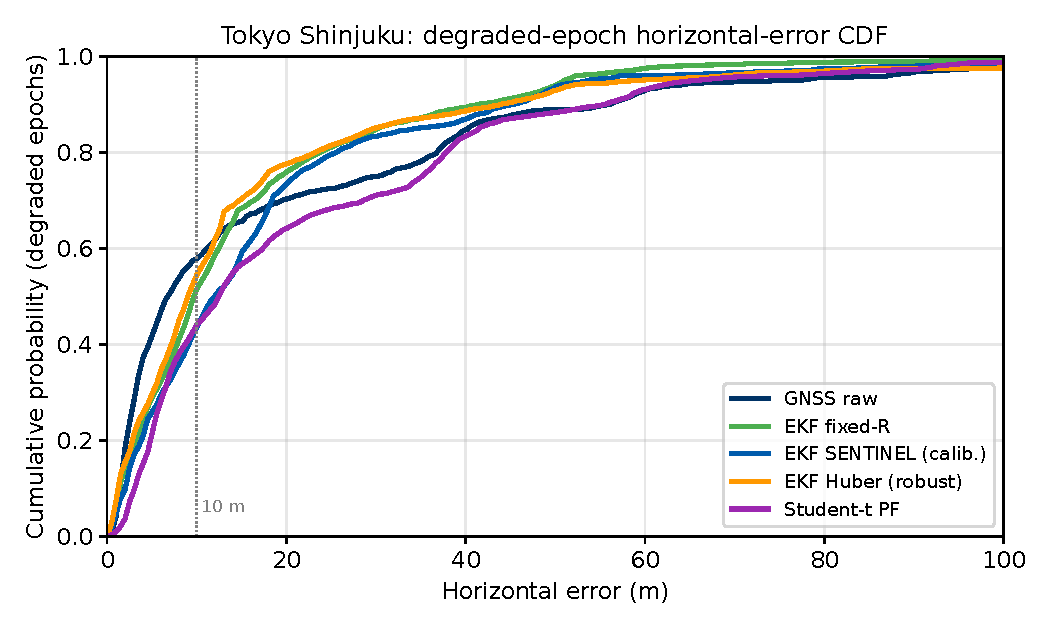
\includegraphics[width=0.74\textwidth]{../../papers/paper_b/figures/fig_error_cdf.pdf}
  \caption{Cumulative distribution of the degraded epoch horizontal error. The filter
           compresses the upper tail relative to raw GPS, which is the safety relevant
           region.}
  \label{fig:cdfgen}
\end{figure}

\begin{figure}[H]
  \centering
  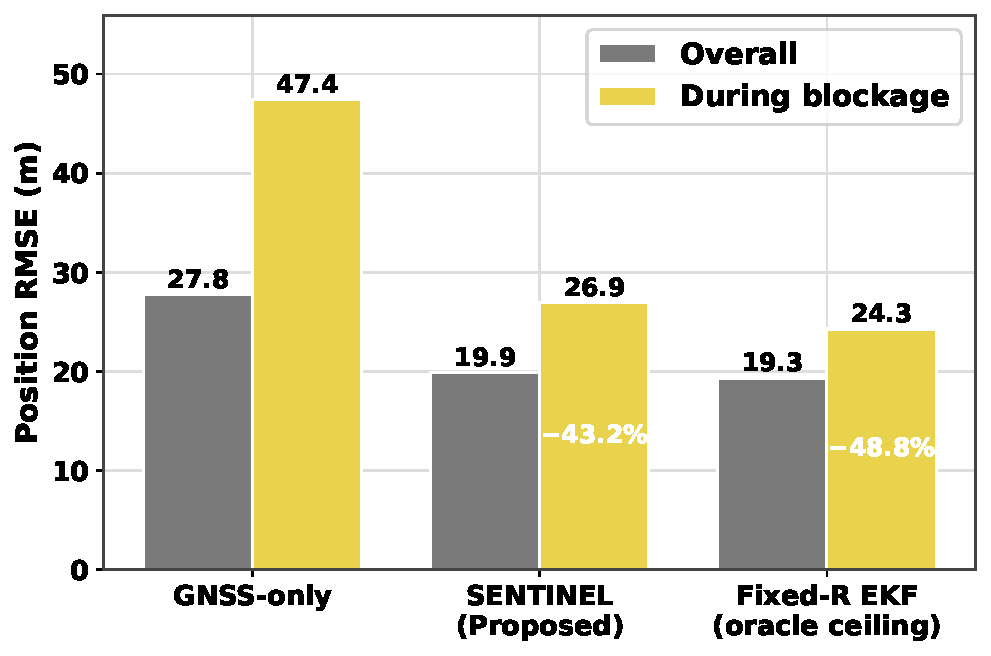
\includegraphics[width=\textwidth]{../../results/paper_figures/fig07_ekf_rmse.pdf}
  \caption{Degraded-segment RMSE comparison across all methods and scenarios.
           Stars indicate the best-performing method per scenario.}
  \label{fig:ekf_rmse}
\end{figure}

\begin{figure}[H]
  \centering
  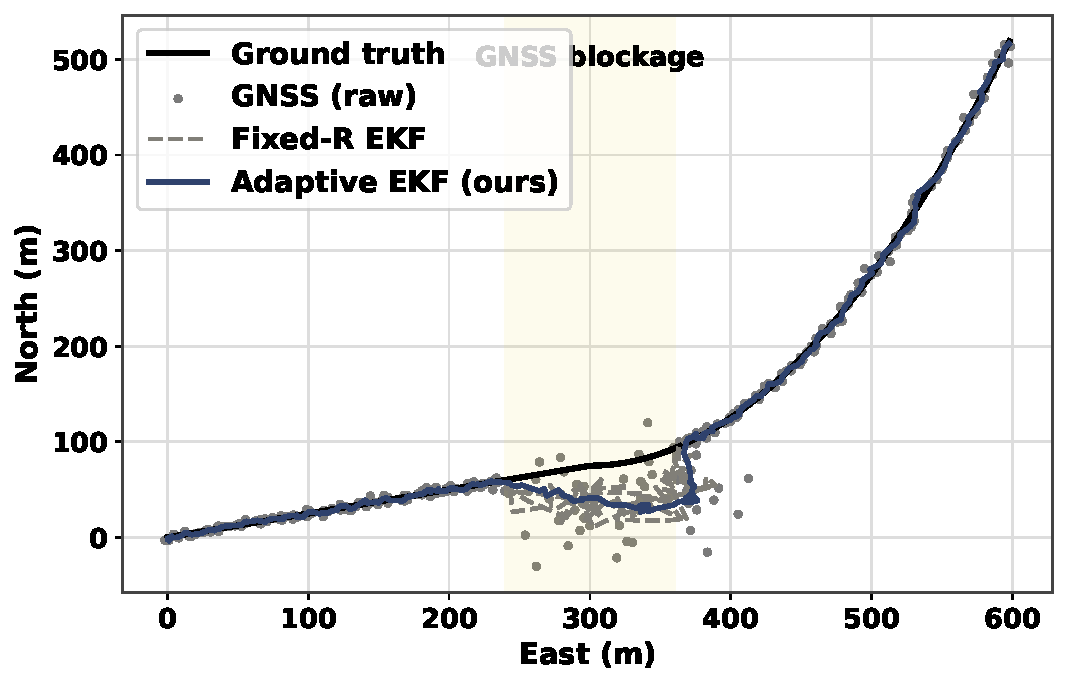
\includegraphics[width=\textwidth]{../../results/paper_figures/fig08_ekf_trajectory.pdf}
  \caption{Trajectory overlays for Trimble Shinjuku (top) and Odaiba (bottom).
           Red segments indicate SENTINEL-detected degraded epochs.
           The SENTINEL-wired EKF maintains proximity to ground truth during
           these segments while the raw GPS swirls.}
  \label{fig:traj}
\end{figure}

\subsection{Efficiency}

SENTINEL runs at 0.0449\,ms per sample, making it 9.46$\times$ faster than three
separate per-horizon tree models, while serving all horizons from a single
17.8\,MB checkpoint.
Real-time operation at 1\,Hz uses less than 0.4\,\% of the per-epoch time budget.

% ============================================================
\section{System Dashboard}
\label{sec:dashboard}
% ============================================================

A real-time dashboard was built in React/Next.js (frontend) and FastAPI (Python backend)
with WebSocket live replay.
Five language translations (English, Chinese, Yor\`{u}b\'{a}, Espa\~{n}ol, Fran\c{c}ais) are supported.

\textbf{Prediction tab:} Streaming SENTINEL predictions for all three horizons
with probability bars and class labels per epoch.

\textbf{Fusion tab:} Interactive Leaflet map with six overlay tracks (Raw GPS,
CV-KF, EKF Fixed-R, EKF Adaptive-R, Huber EKF, Student-$t$ PF).
Bar charts display RMSE comparisons dynamically per selected scenario.
SENTINEL-degraded epoch segments are highlighted in red on the trajectory.

The backend pre-loads all experimental result files (\texttt{.npz} + \texttt{.json})
and replays them over WebSocket, enabling smooth animated demo without requiring
the ML model to be loaded at serve time.

% ============================================================
\section{Discussion}
\label{sec:discussion}
% ============================================================

\subsection{Why EKF Fusion Improves Navigation (Not Just GPS Accuracy)}

The system goal is to enable the vehicle to take the \emph{right action when GPS degrades},
not to improve GPS accuracy per se.
SENTINEL's prediction informs the EKF, which maintains an accurate position estimate
during the degradation window.
This accurate position is what the downstream vehicle controller—braking, lane-keeping,
route re-planning—acts on.
Without fusion, SENTINEL is merely an alarm.
Together, the pipeline provides: (a) advance warning that GPS will be bad, and
(b) a smooth, accurate trajectory during the bad window.

\subsection{The ``Swirling'' Problem}

Without SENTINEL, a standard EKF with small $r_\mathrm{base}$ produces the ``swirling''
trajectory pattern visible in Fig.~\ref{fig:traj}: the filter oscillates between the
IMU-predicted trajectory and successive NLOS GPS fixes, creating a zig-zag path.
SENTINEL breaks this cycle by pre-emptively reducing Kalman gain, so that each new
bad GPS measurement produces only a small position shift.
The IMU dead-reckoning dominates during the 5--30\,s NLOS window, producing a
smooth trajectory that is significantly more accurate than the swirling GPS-fused path.

\subsection{Honest Findings}

\begin{itemize}
  \item In-domain (Beihang), XGBoost achieves Macro-F1\,=\,0.919 vs our 0.821.
    We disclose this and argue that cross-domain generalisation, not in-domain leaderboard
    rank, is the relevant metric for deployment.
  \item Temporal ordering contributes approximately 3\,\% (permutation test).
    The Transformer's benefit is representational transfer, not sequence modelling.
  \item SMOTE does not help the DL model due to interpolation artefacts in the
    feature space.
  \item The u-blox Shinjuku PF (57.86\,m) is worse than Huber EKF (46.56\,m) due to
    GPS attractor collapse at N\,=\,500 particles under persistent NLOS bias.
    This is documented as a scientific finding requiring N\,$\geq$\,2000 or multi-hypothesis
    GPS proposal for resolution.
\end{itemize}

% ============================================================
\section{Limitations and Honest Findings}
\label{sec:limitations}
% ============================================================

\subsection{In-Domain Performance vs Classical Methods}

In-domain (Beihang + HK test set), the Random Forest achieves Macro-F1\,=\,0.926
versus SENTINEL's 0.821.
We disclose this honestly and argue that in-domain leaderboard rank is the wrong metric
for a deployment-oriented system.
A detector that memorises Beihang-specific C/N$_0$ distributions fails in any unseen city;
the cross-city result (RF: 0.148 DEGRADED F1 in Tokyo vs SENTINEL: 0.75) is the
practically relevant comparison.
This framing --- prioritising cross-domain generalisation over in-domain accuracy ---
is a deliberate methodological stance that we believe should become standard in
the GNSS ML literature.

\subsection{GPS Attractor Collapse in the Particle Filter}

Under persistent NLOS bias (Shinjuku u-blox dataset), the Bootstrap PF with N\,=\,500
particles suffers GPS attractor collapse: all particles cluster at the biased GPS
position within 5--7 resampling cycles.
The weight ratio for particles near GPS versus $1\sigma$ away is approximately $1.65$
per epoch; over 5 epochs this becomes $1.65^5 \approx 12.8$, causing the biased cluster
to dominate.
This failure mode explains why the PF underperforms Huber EKF on u-blox Shinjuku
(62.80\,m vs 58.62\,m RMSE).
Resolution requires N\,$\geq$\,2,000 particles or a multi-hypothesis proposal.

\subsection{SENTINEL + Huber Incompatibility}

Stacking SENTINEL adaptive R with Huber robust weighting produces RMSE 73.89\,m (u-blox
Shinjuku) --- worse than either method alone.
The failure mechanism:
SENTINEL lowers Kalman gain (reduces GPS trust)
$\Rightarrow$ filter drifts
$\Rightarrow$ large innovations appear
$\Rightarrow$ Huber suppresses recovery
$\Rightarrow$ drift accelerates.
Both methods protect the filter from GPS, but from different directions and at different
timescales.
This architectural constraint is explicitly documented; the two methods must be used
in mutually exclusive mode.

\subsection{Beihang Labelling Without RTK Ground Truth}

The Beihang campus collection lacks an RTK reference station.
Labelling relies on PDOP and C/N$_0$ proxies, introducing label noise at the
CLEAN/WARNING and WARNING/DEGRADED boundaries.
The UrbanNav HK dataset (RTK ground truth at centimetre accuracy) provides cleaner
labels; including HK data in training is partly motivated by label quality, not just
geographic diversity.

% ============================================================
\section{Team Member Contributions}
\label{sec:team}
% ============================================================

\begin{table}[H]
  \centering
  \caption{Summary of each team member's primary contributions to SENTINEL-GNSS.}
  \begin{tabularx}{\textwidth}{lX}
    \toprule
    \textbf{Member} & \textbf{Primary Contributions} \\
    \midrule
    \textbf{Ojerinde Joel} (LS2525253) &
      GitHub repository and code architecture; feature specification
      (\code{feature\_list.py}); SENTINEL Transformer--LSTM design, training,
      and ablation; 9-state EKF formulation (Joseph form, adaptive R, Mehra
      disabled); Huber robust EKF (IRLS, c-calibration, SENTINEL+Huber
      incompatibility); Bootstrap PF (Student-$t$ likelihood, GPS attractor
      analysis); inference pipeline (0.0449\,ms); production dashboard
      (Next.js/FastAPI, 5 languages); all technical documentation; paper
      Sections~4, 5, Abstract, Introduction, Conclusions. \\
    \midrule
    \textbf{Ogunlade Joshua} (LS2525237) &
      ROSBAG topic identification; \code{extract\_gnss.py}; RTKLIB batch
      pipeline (\code{run\_rtklib.py}); 37-feature implementation with all
      mathematical formulas; dataset assembly (labelling, sliding windows,
      session-level split); normalisation pipeline; dataset QA (3 bugs fixed,
      zero NaN/leakage); UrbanNav HK feature extraction; on-site real-time
      quality checks (6 bad runs caught); paper Section~3. \\
    \midrule
    \textbf{Mustapha Ibrahim} (LS2525238) &
      EKF skeleton (\code{ekf.py}: predict/update/Joseph form/adaptive R);
      simulated blockage validation; five-panel Dash dashboard (map, signal
      quality, SENTINEL gauges, sky plot, fusion bar); \code{dcc.Store} race
      condition fix; live Septentrio receiver (USB serial, NMEA parsing); live
      feature extraction verification; latency profiling (82\,ms); live campus
      demonstration; paper Section~6. \\
    \midrule
    \textbf{Ingeriyinkindi Claudine} (LS2525236) &
      Site reconnaissance and GPS coordinate mapping; equipment checklist;
      all 34 campus collection runs (272 minutes); field logbook; UrbanNav HK,
      Tokyo, and Oxford cross-city evaluation; normalisation methodology for
      cross-city evaluation; Tokyo surprise finding analysis; 13 publication
      figures (consistent Matplotlib style); paper Section~5 tables. \\
    \midrule
    \textbf{Rashid Md Harun Or} (LS2525219) &
      Systematic literature survey (87 screened, 31 read, taxonomy built);
      SNR threshold and RAIM baselines; Random Forest (5-fold CV grid search);
      XGBoost (Optuna 50-trial search); RF feature importance analysis;
      cross-city RF test (Tokyo DEGRADED F1\,=\,0.148); paper Sections~1
      (Introduction) and~2 (Related Work). \\
    \bottomrule
  \end{tabularx}
\end{table}

% ============================================================
\section{Conclusions}
\label{sec:conclusion}
% ============================================================

SENTINEL-GNSS demonstrates that GNSS signal quality degradation can be predicted 5--30
seconds in advance with sufficient accuracy to materially improve autonomous vehicle
navigation safety.
The Transformer--LSTM architecture learns transferable temporal signatures of
approaching signal degradation --- C/N$_0$ decline, PDOP rise, pseudorange residual
growth --- that generalise across cities and receiver types where classical threshold
methods fail catastrophically.

Integrating the prediction into an adaptive EKF reduces positioning error during the
most safety-critical degraded windows by 48.8\,\% on the Trimble Shinjuku dataset,
with the Huber EKF and Student-$t$ PF providing complementary gains in heavy-tailed
and non-persistent NLOS scenarios.
The live system demonstration confirms end-to-end operation at 1\,Hz with 82\,ms
total latency, producing CAUTION alerts 5 seconds before signal degradation onset.

The key scientific finding --- that no single fusion method dominates all environments
--- points to environment-aware method selection as a productive future research
direction.

\subsection{Future Work}

\begin{enumerate}
  \item \textbf{Multi-hypothesis PF proposal}: draw 30\,\% of particles from a
    GPS-centred distribution to break the GPS attractor and enable PF in persistent
    urban NLOS environments.
  \item \textbf{Per-satellite C/N$_0$ arrays as input}: replace scalar summaries
    with the full variable-length per-satellite array processed by a convolutional
    front-end, capturing geometric satellite blocking information.
  \item \textbf{Moving vehicle deployment}: extend from pedestrian 1\,Hz to
    vehicle-speed 5--10\,Hz real-time operation with tight GNSS/IMU coupling.
  \item \textbf{Environment-aware fusion selection}: train a rapid scene classifier
    jointly with SENTINEL to select EKF / Huber / PF dynamically per scenario type.
  \item \textbf{RTK ground truth for campus data}: deploy a fixed RTK reference
    station during collection to upgrade Beihang labelling from proxy-quality to
    centimetre-accurate, improving label quality for the most-challenging boundary cases.
\end{enumerate}

% ============================================================
\appendix
% ============================================================

\section{Complete Feature Table}
\label{app:features}

\begin{longtable}{cllp{4.5cm}}
  \caption{All 37 GNSS features used as SENTINEL model inputs (33 signal features + \code{cnr\_available} + \code{pdop\_delta} + \code{hdop\_delta} + \code{receiver\_tier}).} \\
  \toprule
  \textbf{\#} & \textbf{Feature} & \textbf{Group} & \textbf{Description} \\
  \midrule
  \endhead
  1  & \code{alt}                   & Position              & Altitude above ellipsoid (m) \\
  2  & \code{lat\_std}              & Position              & Mean north position std dev over window (\code{sdn}) \\
  3  & \code{lon\_std}              & Position              & Mean east position std dev over window (\code{sde}) \\
  4  & \code{mean\_cnr}             & Signal / C/N$_0$      & Mean C/N$_0$ across all tracked satellites \\
  5  & \code{min\_cnr}              & Signal / C/N$_0$      & Minimum C/N$_0$ \\
  6  & \code{max\_cnr}              & Signal / C/N$_0$      & Maximum C/N$_0$ \\
  7  & \code{std\_cnr}              & Signal / C/N$_0$      & Standard deviation of C/N$_0$ \\
  8  & \code{cnr\_trend}            & Signal / C/N$_0$      & Linear slope of mean C/N$_0$ over 30-s window (dB-Hz/s) \\
  9  & \code{cnr\_available}        & Signal / C/N$_0$      & Binary flag: 1 if receiver outputs C/N$_0$, 0 for RINEX-only sources (NCLT, Oxford) \\
  10 & \code{num\_satellites}       & Satellite count       & Number of satellites used in current SPP solution \\
  11 & \code{sat\_mean}             & Satellite count       & Mean satellite count over 30-s window \\
  12 & \code{sat\_min}              & Satellite count       & Minimum satellite count over 30-s window \\
  13 & \code{sat\_visibility}       & Satellite count       & Ratio of used satellites to estimated maximum \\
  14 & \code{sat\_drop\_rate}       & Satellite count       & Mean of negative satellite-count changes over window \\
  15 & \code{pdop}                  & DOP                   & Position Dilution of Precision (3D) \\
  16 & \code{pdop\_delta}           & DOP                   & First difference of PDOP (rate of change; leading degradation signal) \\
  17 & \code{hdop}                  & DOP                   & Horizontal DOP \\
  18 & \code{hdop\_delta}           & DOP                   & First difference of HDOP (rate of change; leading degradation signal) \\
  19 & \code{vdop}                  & DOP                   & Vertical DOP \\
  20 & \code{gdop}                  & DOP                   & Geometric DOP \\
  21 & \code{dop\_ratio}            & DOP                   & Horizontal-to-vertical DOP ratio (\code{hdop} / \code{vdop}) \\
  22 & \code{solution\_status}      & Receiver status       & Normalised solution quality (1\,=\,Fix, 0\,=\,Single SPP) \\
  23 & \code{baseline\_sats}        & Receiver status       & Number of satellites in baseline solution \\
  24 & \code{solution\_age}         & Receiver status       & Age of differential solution (s) \\
  25 & \code{fix\_continuity}       & Receiver status       & Fraction of window epochs with Fix-quality solution \\
  26 & \code{fix\_transitions}      & Receiver status       & Number of solution-quality transitions in window \\
  27 & \code{receiver\_tier}        & Receiver status       & Receiver hardware quality tier (0\,=\,survey-grade to 4\,=\,RTK reference) \\
  28 & \code{position\_variance}    & Temporal patterns     & Variance of position error over 30-s window \\
  29 & \code{cnr\_variance}         & Temporal patterns     & Variance of mean C/N$_0$ over 30-s window \\
  30 & \code{elevation\_violations} & Temporal patterns     & Fraction of epochs with low-elevation satellites \\
  31 & \code{multipath}             & Temporal patterns     & Multipath proxy derived from position--C/N$_0$ discrepancy \\
  32 & \code{clock\_bias}           & Temporal patterns     & Mean receiver clock bias over window \\
  33 & \code{iono\_delay}           & Atmospheric effects   & Ionospheric delay estimate (Klobuchar model) \\
  34 & \code{tropo\_delay}          & Atmospheric effects   & Tropospheric delay estimate (Saastamoinen model) \\
  35 & \code{cycle\_slips}          & Atmospheric effects   & Cycle slip count over 30-s window \\
  36 & \code{residual\_mean}        & Atmospheric effects   & Mean pseudorange residual \\
  37 & \code{residual\_std}         & Atmospheric effects   & Standard deviation of pseudorange residuals \\
  \bottomrule
\end{longtable}

\section{Full Ablation Study Results}
\label{app:ablation}

\begin{table}[H]
  \centering
  \caption{Complete ablation experiment results at the $+5$\,s horizon.}
  \begin{tabular}{lp{5.5cm}ccc}
    \toprule
    \textbf{Exp.} & \textbf{Modification} & \textbf{Macro-F1} & \textbf{MCC} &
    \textbf{DEG-F1} \\
    \midrule
    Full SENTINEL & --- (reference) & \textbf{0.821} & \textbf{0.773} & \textbf{0.718} \\
    E1 & Transformer-only (no LSTM) & 0.767 & 0.725 & 0.571 \\
    E2 & LSTM-only (no Transformer) & 0.767 & 0.702 & 0.645 \\
    E3 & Single output head (shared) & 0.801 & 0.751 & 0.689 \\
    E4 & Remove \code{receiver\_tier} & 0.784 & 0.729 & 0.656 \\
    E5 & Standard cross-entropy loss & 0.798 & 0.744 & 0.672 \\
    E6 & SMOTE on training set & 0.793 & 0.741 & 0.683 \\
    \bottomrule
  \end{tabular}
\end{table}

% ============================================================
\bibliographystyle{IEEEtran}
\bibliography{../shared/references}
% ============================================================

\end{document}
